\documentclass[final,5p,times,twocolumn]{elsarticle}
\usepackage{amsmath,amssymb,amsfonts,amsthm}
\usepackage{graphicx,booktabs,multirow,siunitx,enumitem,placeins,microtype,textcomp,float}
\usepackage{algorithm,algpseudocode}
\usepackage[hidelinks]{hyperref}
\sisetup{detect-all,range-phrase=--,range-units=single}
\newtheorem{theorem}{Theorem}\newtheorem{lemma}{Lemma}\newtheorem{proposition}{Proposition}\newtheorem{definition}{Definition}\newtheorem{assumption}{Assumption}\newtheorem{fact}{Fact}
\newcommand{\gth}{g_\theta}\newcommand{\thsp}{\theta_{\mathrm{sp}}}\newcommand{\lf}{\Lambda}

% ---- numbers ----
%% generated by code/hot/numbers.py
\newcommand{\ablBestL}{32}
\newcommand{\ablBoneLf}{0.92}
\newcommand{\ablBoneReached}{58}
\newcommand{\ablBoneReachedF}{33}
\newcommand{\ablBoneTmed}{4.7}
\newcommand{\ablBoneViol}{0.1}
\newcommand{\ablDsmallLf}{0.93}
\newcommand{\ablDsmallReached}{65}
\newcommand{\ablDsmallReachedF}{60}
\newcommand{\ablDsmallTmed}{5.0}
\newcommand{\ablDsmallViol}{0.1}
\newcommand{\ablFullLf}{0.92}
\newcommand{\ablFullReached}{98}
\newcommand{\ablFullReachedF}{87}
\newcommand{\ablFullTmed}{4.7}
\newcommand{\ablFullViol}{1.8}
\newcommand{\ablLsmallLf}{0.94}
\newcommand{\ablLsmallReached}{63}
\newcommand{\ablLsmallReachedF}{33}
\newcommand{\ablLsmallTmed}{4.5}
\newcommand{\ablLsmallViol}{2.1}
\newcommand{\ablLstmLf}{0.95}
\newcommand{\ablLstmReached}{88}
\newcommand{\ablLstmReachedF}{80}
\newcommand{\ablLstmTmed}{6.1}
\newcommand{\ablLstmViol}{0.1}
\newcommand{\ablMlpLf}{0.92}
\newcommand{\ablMlpReached}{100}
\newcommand{\ablMlpReachedF}{97}
\newcommand{\ablMlpTmed}{4.4}
\newcommand{\ablMlpViol}{0.1}
\newcommand{\ablNoAuxLf}{0.89}
\newcommand{\ablNoAuxReached}{73}
\newcommand{\ablNoAuxReachedF}{55}
\newcommand{\ablNoAuxRtwo}{0.37}
\newcommand{\ablNoAuxT}{6.5}
\newcommand{\ablNoAuxTmed}{5.0}
\newcommand{\ablNoAuxViol}{2.8}
\newcommand{\ablNoPhysLf}{0.93}
\newcommand{\ablNoPhysReached}{40}
\newcommand{\ablNoPhysReachedF}{28}
\newcommand{\ablNoPhysT}{5.0}
\newcommand{\ablNoPhysTmed}{5.0}
\newcommand{\ablNoPhysViol}{1.1}
\newcommand{\bestOtherCrossName}{the threshold rule}
\newcommand{\bestOtherCrossRank}{3.82}
\newcommand{\hotBackAl}{0.6}
\newcommand{\hotBackEnergy}{4.51}
\newcommand{\hotBackInterv}{0}
\newcommand{\hotBackLf}{0.96}
\newcommand{\hotBackT}{4.7}
\newcommand{\hotBackUpd}{400}
\newcommand{\hotCheckMaxMs}{37}
\newcommand{\hotCheckMs}{28}
\newcommand{\hotCrossBackInterv}{0.3}
\newcommand{\hotCrossBackIntervPct}{0.1}
\newcommand{\hotCrossBackN}{100}
\newcommand{\hotCrossBackReached}{89}
\newcommand{\hotCrossBackStalledNoInt}{4}
\newcommand{\hotCrossBackStalledUnver}{7}
\newcommand{\hotCrossBackTmed}{4.9}
\newcommand{\hotCrossBackUnver}{0.3}
\newcommand{\hotCrossFrontInterv}{12.9}
\newcommand{\hotCrossFrontIntervPct}{3.2}
\newcommand{\hotCrossFrontN}{100}
\newcommand{\hotCrossFrontReached}{88}
\newcommand{\hotCrossFrontStalledNoInt}{0}
\newcommand{\hotCrossFrontStalledUnver}{5}
\newcommand{\hotCrossFrontTmed}{4.7}
\newcommand{\hotCrossFrontUnver}{3.8}
\newcommand{\hotCrossInterv}{2}
\newcommand{\hotCrossLf}{0.94}
\newcommand{\hotCrossRank}{3.24}
\newcommand{\hotCrossReached}{88\%}
\newcommand{\hotCrossT}{5.5}
\newcommand{\hotCrossViol}{0.0}
\newcommand{\hotEvalMs}{0.6}
\newcommand{\hotEvalUs}{?}
\newcommand{\hotFrontAl}{-0.2}
\newcommand{\hotFrontEnergy}{4.21}
\newcommand{\hotFrontInterv}{2}
\newcommand{\hotFrontLf}{0.94}
\newcommand{\hotFrontT}{4.5}
\newcommand{\hotFrontUpd}{400}
\newcommand{\hotGustHalfAl}{4.0}
\newcommand{\hotGustHalfInterv}{7}
\newcommand{\hotGustHalfLf}{0.78}
\newcommand{\hotGustHalfReached}{19}
\newcommand{\hotGustHalfViol}{2.9}
\newcommand{\hotGustInterv}{12}
\newcommand{\hotGustLf}{0.87}
\newcommand{\hotGustOneAl}{6.4}
\newcommand{\hotGustOneHalfAl}{8.4}
\newcommand{\hotGustOneHalfInterv}{19}
\newcommand{\hotGustOneHalfLf}{0.70}
\newcommand{\hotGustOneHalfReached}{17}
\newcommand{\hotGustOneHalfViol}{15.4}
\newcommand{\hotGustOneInterv}{20}
\newcommand{\hotGustOneLf}{0.68}
\newcommand{\hotGustOneReached}{15}
\newcommand{\hotGustOneViol}{15.2}
\newcommand{\hotGustQtrAl}{1.5}
\newcommand{\hotGustQtrInterv}{1}
\newcommand{\hotGustQtrLf}{0.85}
\newcommand{\hotGustQtrReached}{20}
\newcommand{\hotGustQtrViol}{0.0}
\newcommand{\hotGustReached}{89\%}
\newcommand{\hotGustStrongInterv}{20}
\newcommand{\hotGustStrongUnverShare}{96}
\newcommand{\hotGustStrongViol}{15}
\newcommand{\hotGustT}{5.6}
\newcommand{\hotGustViol}{8.4}
\newcommand{\hotNoiseHalfBackReached}{10}
\newcommand{\hotNoiseHalfBackTmed}{4.7}
\newcommand{\hotNoiseHalfFrontReached}{10}
\newcommand{\hotNoiseHalfFrontTmed}{5.3}
\newcommand{\hotNoiseInterv}{1}
\newcommand{\hotNoiseLf}{0.95}
\newcommand{\hotNoiseOneBackReached}{9}
\newcommand{\hotNoiseOneBackTmed}{4.7}
\newcommand{\hotNoiseOneFrontReached}{10}
\newcommand{\hotNoiseOneFrontTmed}{8.9}
\newcommand{\hotNoiseReached}{87\%}
\newcommand{\hotNoiseT}{6.6}
\newcommand{\hotNoiseTwoBackReached}{9}
\newcommand{\hotNoiseTwoBackTmed}{5.3}
\newcommand{\hotNoiseTwoFrontReached}{4}
\newcommand{\hotNoiseTwoFrontTmed}{11.7}
\newcommand{\hotNoiseViol}{0.0}
\newcommand{\hotOutBackInterv}{11.3}
\newcommand{\hotOutBackIntervPct}{2.8}
\newcommand{\hotOutBackN}{50}
\newcommand{\hotOutBackReached}{33}
\newcommand{\hotOutBackStalledNoInt}{8}
\newcommand{\hotOutBackStalledUnver}{9}
\newcommand{\hotOutBackTmed}{5.5}
\newcommand{\hotOutBackUnver}{11.3}
\newcommand{\hotOutFrontInterv}{29.4}
\newcommand{\hotOutFrontIntervPct}{7.3}
\newcommand{\hotOutFrontN}{50}
\newcommand{\hotOutFrontReached}{33}
\newcommand{\hotOutFrontStalledNoInt}{6}
\newcommand{\hotOutFrontStalledUnver}{10}
\newcommand{\hotOutFrontTmed}{4.5}
\newcommand{\hotOutFrontUnver}{15.1}
\newcommand{\hotOutInterv}{5}
\newcommand{\hotOutLf}{0.92}
\newcommand{\hotOutReached}{66\%}
\newcommand{\hotOutT}{6.8}
\newcommand{\hotOutViol}{0.0}
\newcommand{\hotReplayBackAl}{2.5}
\newcommand{\hotReplayBackInterv}{3}
\newcommand{\hotReplayBackLf}{0.83}
\newcommand{\hotReplayBackT}{4.8}
\newcommand{\hotReplayBackUnver}{3}
\newcommand{\hotReplayFrontAl}{-1.1}
\newcommand{\hotReplayFrontInterv}{21}
\newcommand{\hotReplayFrontLf}{0.97}
\newcommand{\hotReplayFrontT}{?}
\newcommand{\hotnfBackAl}{0.6}
\newcommand{\hotnfBackEnergy}{4.51}
\newcommand{\hotnfBackInterv}{?}
\newcommand{\hotnfBackLf}{0.96}
\newcommand{\hotnfBackT}{4.7}
\newcommand{\hotnfBackUpd}{400}
\newcommand{\hotnfCrossLf}{0.92}
\newcommand{\hotnfCrossRank}{1.89}
\newcommand{\hotnfCrossReached}{98\%}
\newcommand{\hotnfCrossT}{5.2}
\newcommand{\hotnfCrossViol}{1.6}
\newcommand{\hotnfFrontAl}{-0.2}
\newcommand{\hotnfFrontEnergy}{4.17}
\newcommand{\hotnfFrontInterv}{?}
\newcommand{\hotnfFrontLf}{0.94}
\newcommand{\hotnfFrontT}{4.0}
\newcommand{\hotnfFrontUpd}{400}
\newcommand{\interpAttMax}{0.032}
\newcommand{\interpAttMin}{0.028}
\newcommand{\interpAttUniform}{0.031}
\newcommand{\interpErrMean}{0.243}
\newcommand{\interpRtwoBetaR}{0.84}
\newcommand{\interpRtwoCDzero}{0.50}
\newcommand{\interpRtwoCLa}{0.44}
\newcommand{\interpRtwoCLzero}{0.83}
\newcommand{\interpRtwoGth}{0.30}
\newcommand{\interpRtwoKappa}{0.77}
\newcommand{\interpRtwoKdrag}{0.11}
\newcommand{\interpRtwoLamR}{0.03}
\newcommand{\interpRtwoMean}{0.42}
\newcommand{\interpShrinkBetaR}{0.08}
\newcommand{\interpShrinkCDzero}{0.11}
\newcommand{\interpShrinkCLa}{0.14}
\newcommand{\interpShrinkCLzero}{0.04}
\newcommand{\interpShrinkGth}{0.01}
\newcommand{\interpShrinkKappa}{0.01}
\newcommand{\interpShrinkKdrag}{0.02}
\newcommand{\interpShrinkLamR}{0.03}
\newcommand{\interpTBetaR}{1.5}
\newcommand{\interpTCDzero}{10.0}
\newcommand{\interpTCLa}{7.0}
\newcommand{\interpTCLzero}{2.5}
\newcommand{\interpTGth}{3.5}
\newcommand{\interpTKappa}{1.5}
\newcommand{\interpTKdrag}{6.0}
\newcommand{\interpTLamR}{5.0}
\newcommand{\interpTrBetaR}{front}
\newcommand{\interpTrCDzero}{front}
\newcommand{\interpTrCLa}{front}
\newcommand{\interpTrCLzero}{back}
\newcommand{\interpTrGth}{front}
\newcommand{\interpTrKappa}{back}
\newcommand{\interpTrKdrag}{back}
\newcommand{\interpTrLamR}{back}
\newcommand{\lstmBackAl}{-0.8}
\newcommand{\lstmBackEnergy}{4.87}
\newcommand{\lstmBackInterv}{0}
\newcommand{\lstmBackLf}{0.94}
\newcommand{\lstmBackT}{5.2}
\newcommand{\lstmBackUpd}{400}
\newcommand{\lstmCrossViol}{?}
\newcommand{\lstmFrontAl}{-0.0}
\newcommand{\lstmFrontEnergy}{4.16}
\newcommand{\lstmFrontInterv}{8}
\newcommand{\lstmFrontLf}{0.97}
\newcommand{\lstmFrontT}{6.6}
\newcommand{\lstmFrontUpd}{400}
\newcommand{\maxOtherCrossViol}{36.6}
\newcommand{\mlpBackAl}{1.9}
\newcommand{\mlpBackEnergy}{4.51}
\newcommand{\mlpBackInterv}{2}
\newcommand{\mlpBackLf}{0.92}
\newcommand{\mlpBackT}{6.9}
\newcommand{\mlpBackUpd}{400}
\newcommand{\mlpCrossViol}{?}
\newcommand{\mlpFrontAl}{-0.1}
\newcommand{\mlpFrontEnergy}{4.02}
\newcommand{\mlpFrontInterv}{5}
\newcommand{\mlpFrontLf}{0.92}
\newcommand{\mlpFrontT}{3.8}
\newcommand{\mlpFrontUpd}{400}
\newcommand{\mpcBackAl}{0.3}
\newcommand{\mpcBackEnergy}{3.60}
\newcommand{\mpcBackInterv}{?}
\newcommand{\mpcBackLf}{1.00}
\newcommand{\mpcBackT}{19.5}
\newcommand{\mpcBackUpd}{400}
\newcommand{\mpcCrossLf}{0.96}
\newcommand{\mpcCrossRank}{7.28}
\newcommand{\mpcCrossReached}{50\%}
\newcommand{\mpcCrossT}{15.1}
\newcommand{\mpcCrossViol}{0.0}
\newcommand{\mpcFrontAl}{0.4}
\newcommand{\mpcFrontEnergy}{3.39}
\newcommand{\mpcFrontInterv}{?}
\newcommand{\mpcFrontLf}{1.00}
\newcommand{\mpcFrontT}{18.4}
\newcommand{\mpcFrontUpd}{400}
\newcommand{\mpcStepMs}{518}
\newcommand{\numAR}{6.85}
\newcommand{\numAblPlants}{30}
\newcommand{\numAmax}{1.0}
\newcommand{\numBatch}{32}
\newcommand{\numBlocks}{2}
\newcommand{\numCalHi}{0.5}
\newcommand{\numCalLo}{-9}
\newcommand{\numCgam}{3}
\newcommand{\numCgd}{0.05}
\newcommand{\numClfHi}{1.07}
\newcommand{\numClfLo}{0.93}
\newcommand{\numCross}{100}
\newcommand{\numCvHi}{16}
\newcommand{\numCvLo}{5}
\newcommand{\numCvd}{0.6}
\newcommand{\numD}{48}
\newcommand{\numEps}{0.4\ \mathrm{m/s},\ 1^\circ,\ 1^\circ,\ 1.5\ \mathrm N,\ 4\ \mathrm N}
\newcommand{\numFriedmanN}{40}
\newcommand{\numGdLim}{0.3}
\newcommand{\numH}{200}
\newcommand{\numHeads}{4}
\newcommand{\numIters}{800}
\newcommand{\numKL}{0.25}
\newcommand{\numKc}{6}
\newcommand{\numKcGain}{0.17}
\newcommand{\numKcRho}{0.97}
\newcommand{\numKgam}{0.4}
\newcommand{\numKr}{10}
\newcommand{\numKrGain}{0.17}
\newcommand{\numKrRho}{0.89}
\newcommand{\numKv}{0.5}
\newcommand{\numL}{32}
\newcommand{\numLr}{$2\times10^{-4}$}
\newcommand{\numMargins}{0.02,\ 0^\circ,\ 0^\circ,\ 0^\circ,\ 1^\circ,\ 1^\circ,\ 0.02,\ 0.3}
\newcommand{\numOutbox}{50}
\newcommand{\numParams}{79,101}
\newcommand{\numPlantsFull}{1088}
\newcommand{\numPlantsOnline}{128}
\newcommand{\numRhi}{0.15}
\newcommand{\numRlo}{-0.15}
\newcommand{\numSamplesOnline}{32}
\newcommand{\numSettleFail}{0}
\newcommand{\numSettlePairs}{23,914}
\newcommand{\numSettleWorst}{0.011}
\newcommand{\numTauB}{0.75}
\newcommand{\numVbhi}{15.5}
\newcommand{\numVblo}{6}
\newcommand{\numWA}{1}
\newcommand{\numWB}{2}
\newcommand{\numWE}{0.2}
\newcommand{\numWS}{0.3}
\newcommand{\pidBackAl}{-0.0}
\newcommand{\pidBackEnergy}{3.56}
\newcommand{\pidBackInterv}{?}
\newcommand{\pidBackLf}{0.98}
\newcommand{\pidBackT}{14.5}
\newcommand{\pidBackUpd}{400}
\newcommand{\pidCrossLf}{0.97}
\newcommand{\pidCrossRank}{5.06}
\newcommand{\pidCrossReached}{95\%}
\newcommand{\pidCrossT}{9.7}
\newcommand{\pidCrossViol}{0.0}
\newcommand{\pidFrontAl}{-0.0}
\newcommand{\pidFrontEnergy}{3.32}
\newcommand{\pidFrontInterv}{?}
\newcommand{\pidFrontLf}{0.99}
\newcommand{\pidFrontT}{5.2}
\newcommand{\pidFrontUpd}{400}
\newcommand{\pidGustHalfLf}{0.73}
\newcommand{\pidGustHalfViol}{0.1}
\newcommand{\pidGustLf}{0.84}
\newcommand{\pidGustOneHalfLf}{0.34}
\newcommand{\pidGustOneHalfViol}{9.3}
\newcommand{\pidGustOneLf}{0.53}
\newcommand{\pidGustOneViol}{5.0}
\newcommand{\pidGustQtrLf}{0.86}
\newcommand{\pidGustQtrViol}{0.0}
\newcommand{\pidGustReached}{84\%}
\newcommand{\pidGustT}{8.9}
\newcommand{\pidGustViol}{3.6}
\newcommand{\pidNoiseLf}{0.97}
\newcommand{\pidNoiseReached}{100\%}
\newcommand{\pidNoiseT}{9.8}
\newcommand{\pidNoiseViol}{0.0}
\newcommand{\pidOutLf}{0.95}
\newcommand{\pidOutReached}{78\%}
\newcommand{\pidOutT}{9.7}
\newcommand{\pidOutViol}{0.0}
\newcommand{\pidUs}{77}
\newcommand{\ppoBackAl}{3.2}
\newcommand{\ppoBackEnergy}{4.03}
\newcommand{\ppoBackInterv}{?}
\newcommand{\ppoBackLf}{0.94}
\newcommand{\ppoBackT}{8.2}
\newcommand{\ppoBackUpd}{400}
\newcommand{\ppoCrossLf}{0.60}
\newcommand{\ppoCrossRank}{5.61}
\newcommand{\ppoCrossReached}{50\%}
\newcommand{\ppoCrossT}{8.3}
\newcommand{\ppoCrossViol}{36.6}
\newcommand{\ppoFrontAl}{1.2}
\newcommand{\ppoFrontEnergy}{8.94}
\newcommand{\ppoFrontInterv}{?}
\newcommand{\ppoFrontLf}{0.32}
\newcommand{\ppoFrontT}{?}
\newcommand{\ppoFrontUpd}{400}
\newcommand{\ppoGustLf}{0.54}
\newcommand{\ppoGustReached}{50\%}
\newcommand{\ppoGustT}{8.3}
\newcommand{\ppoGustViol}{37.4}
\newcommand{\ppoNoiseLf}{0.62}
\newcommand{\ppoNoiseReached}{50\%}
\newcommand{\ppoNoiseT}{8.2}
\newcommand{\ppoNoiseViol}{35.9}
\newcommand{\ppoOutLf}{-3.31}
\newcommand{\ppoOutReached}{48\%}
\newcommand{\ppoOutT}{8.8}
\newcommand{\ppoOutViol}{38.4}
\newcommand{\sacBackAl}{4.7}
\newcommand{\sacBackEnergy}{4.30}
\newcommand{\sacBackInterv}{?}
\newcommand{\sacBackLf}{0.94}
\newcommand{\sacBackT}{4.9}
\newcommand{\sacBackUpd}{400}
\newcommand{\sacCrossLf}{0.91}
\newcommand{\sacCrossRank}{3.86}
\newcommand{\sacCrossReached}{87\%}
\newcommand{\sacCrossT}{5.9}
\newcommand{\sacCrossViol}{0.3}
\newcommand{\sacFrontAl}{-0.3}
\newcommand{\sacFrontEnergy}{3.01}
\newcommand{\sacFrontInterv}{?}
\newcommand{\sacFrontLf}{0.91}
\newcommand{\sacFrontT}{7.3}
\newcommand{\sacFrontUpd}{400}
\newcommand{\sacGustHalfLf}{0.67}
\newcommand{\sacGustHalfViol}{1.8}
\newcommand{\sacGustLf}{0.79}
\newcommand{\sacGustOneHalfLf}{0.22}
\newcommand{\sacGustOneHalfViol}{13.1}
\newcommand{\sacGustOneLf}{0.39}
\newcommand{\sacGustOneViol}{8.4}
\newcommand{\sacGustQtrLf}{0.83}
\newcommand{\sacGustQtrViol}{0.5}
\newcommand{\sacGustReached}{100\%}
\newcommand{\sacGustT}{5.9}
\newcommand{\sacGustViol}{6.0}
\newcommand{\sacNoiseLf}{0.91}
\newcommand{\sacNoiseReached}{100\%}
\newcommand{\sacNoiseT}{6.0}
\newcommand{\sacNoiseViol}{0.1}
\newcommand{\sacOutLf}{0.90}
\newcommand{\sacOutReached}{84\%}
\newcommand{\sacOutT}{6.1}
\newcommand{\sacOutViol}{0.3}
\newcommand{\schBackAl}{0.8}
\newcommand{\schBackEnergy}{3.77}
\newcommand{\schBackInterv}{?}
\newcommand{\schBackLf}{0.98}
\newcommand{\schBackT}{11.3}
\newcommand{\schBackUpd}{400}
\newcommand{\schCrossLf}{0.97}
\newcommand{\schCrossRank}{5.24}
\newcommand{\schCrossReached}{87\%}
\newcommand{\schCrossT}{9.4}
\newcommand{\schCrossViol}{2.5}
\newcommand{\schFrontAl}{-0.0}
\newcommand{\schFrontEnergy}{3.38}
\newcommand{\schFrontInterv}{?}
\newcommand{\schFrontLf}{0.99}
\newcommand{\schFrontT}{7.2}
\newcommand{\schFrontUpd}{400}
\newcommand{\schGustHalfLf}{0.72}
\newcommand{\schGustHalfViol}{1.8}
\newcommand{\schGustLf}{0.83}
\newcommand{\schGustOneHalfLf}{0.42}
\newcommand{\schGustOneHalfViol}{23.6}
\newcommand{\schGustOneLf}{0.51}
\newcommand{\schGustOneViol}{14.0}
\newcommand{\schGustQtrLf}{0.85}
\newcommand{\schGustQtrViol}{0.0}
\newcommand{\schGustReached}{96\%}
\newcommand{\schGustT}{9.8}
\newcommand{\schGustViol}{9.8}
\newcommand{\schNoiseLf}{0.97}
\newcommand{\schNoiseReached}{100\%}
\newcommand{\schNoiseT}{9.2}
\newcommand{\schNoiseViol}{0.0}
\newcommand{\schOutLf}{0.95}
\newcommand{\schOutReached}{78\%}
\newcommand{\schOutT}{9.8}
\newcommand{\schOutViol}{4.3}
\newcommand{\schUs}{68}
\newcommand{\silBackAlMax}{-2.7}
\newcommand{\silBackAlMin}{-6.6}
\newcommand{\silBackGam}{3.9}
\newcommand{\silBackInterv}{0}
\newcommand{\silBackLf}{0.98}
\newcommand{\silBackT}{29.2}
\newcommand{\silBackUpd}{527}
\newcommand{\silFrontAlMax}{2.5}
\newcommand{\silFrontAlMin}{-7.2}
\newcommand{\silFrontGam}{3.6}
\newcommand{\silFrontInterv}{0}
\newcommand{\silFrontLf}{1.00}
\newcommand{\silFrontT}{17.5}
\newcommand{\silFrontUpd}{377}
\newcommand{\silUpdMs}{79}
\newcommand{\thrBackAl}{3.2}
\newcommand{\thrBackEnergy}{3.51}
\newcommand{\thrBackInterv}{?}
\newcommand{\thrBackLf}{0.95}
\newcommand{\thrBackT}{12.2}
\newcommand{\thrBackUpd}{400}
\newcommand{\thrCrossLf}{0.88}
\newcommand{\thrCrossRank}{3.82}
\newcommand{\thrCrossReached}{96\%}
\newcommand{\thrCrossT}{8.0}
\newcommand{\thrCrossViol}{1.6}
\newcommand{\thrFrontAl}{-0.0}
\newcommand{\thrFrontEnergy}{2.99}
\newcommand{\thrFrontInterv}{?}
\newcommand{\thrFrontLf}{0.84}
\newcommand{\thrFrontT}{4.6}
\newcommand{\thrFrontUpd}{400}
\newcommand{\thrGustHalfLf}{0.67}
\newcommand{\thrGustHalfViol}{1.4}
\newcommand{\thrGustLf}{0.78}
\newcommand{\thrGustOneHalfLf}{0.25}
\newcommand{\thrGustOneHalfViol}{23.7}
\newcommand{\thrGustOneLf}{0.38}
\newcommand{\thrGustOneViol}{12.3}
\newcommand{\thrGustQtrLf}{0.76}
\newcommand{\thrGustQtrViol}{0.0}
\newcommand{\thrGustReached}{96\%}
\newcommand{\thrGustT}{8.3}
\newcommand{\thrGustViol}{9.3}
\newcommand{\thrNoiseLf}{0.89}
\newcommand{\thrNoiseReached}{100\%}
\newcommand{\thrNoiseT}{8.3}
\newcommand{\thrNoiseViol}{0.0}
\newcommand{\thrOutLf}{0.87}
\newcommand{\thrOutReached}{89\%}
\newcommand{\thrOutT}{7.9}
\newcommand{\thrOutViol}{1.3}
\newcommand{\thrUs}{12}
\newcommand{\trainAux}{1.65}
\newcommand{\trainBarrierDrop}{a factor of 0}
\newcommand{\trainReached}{0.97}
\newcommand{\trainWallMin}{60}


\journal{Neurocomputing}
\setcounter{topnumber}{3}\setcounter{bottomnumber}{2}\setcounter{totalnumber}{5}\setcounter{dbltopnumber}{3}\renewcommand{\topfraction}{0.95}\renewcommand{\dbltopfraction}{0.95}\renewcommand{\bottomfraction}{0.6}\renewcommand{\textfraction}{0.05}\renewcommand{\floatpagefraction}{0.75}\renewcommand{\dblfloatpagefraction}{0.75}
\begin{document}
\begin{frontmatter}
\title{Safe hand-off control of a quadplane VTOL across an uncertain plant family with a history-conditioned transformer}
\author[tt]{Md Nur-A-Adam Dony\corref{cor}}
\ead{mdony42@tntech.edu}
\cortext[cor]{Corresponding author.}
\affiliation[tt]{organization={Department of Electrical and Computer Engineering, Tennessee Technological University}, city={Cookeville}, state={TN}, postcode={38505}, country={USA}}
\author[kl]{Md Azizul Islam}
\affiliation[kl]{organization={KaiLab LLC}, city={Sugar Land}, state={TX}, postcode={77479}, country={USA}}
\begin{abstract}

% ---- abstract ----
The hand-off of a quadplane between its lift rotors and its wing decides whether the aircraft flies or falls, and open-source autopilots decide it by an airspeed threshold. This article introduces HOT, a history-conditioned transformer that reads the last $L$ autopilot samples, infers the aircraft it is flying through a context token, and commands the pitch setpoint, the pusher and the rotors through a bounded head. The policy is trained by backpropagation through a differentiable model identified from the flight log of an \SI{8}{kg} quadplane, under domain randomisation over ten plant parameters, gusts and noise. A lift-safety module rolls a backup manoeuvre out over the vertices of the parameter box and the plants consistent with the observed transitions, and accepts the network command only if every rollout keeps the lift margin, the angle of attack, the flight path and the sink rate within bounds and settles into level flight. Recursive feasibility and constraint satisfaction over the verified plant set are proved, and the context token is shown to resolve the plant parameters while the responses that reveal them are inside the window. On \numCross{} unseen plants, outside the box, under gusts and noise, from states recorded in flight and with the PX4 firmware in the loop, HOT is compared with nine controllers, including model predictive control and reinforcement learning. It completes the front transition in \hotFrontT{}~s with the lift fraction never below \hotFrontLf{}, keeps every constraint on every unseen plant, and evaluates in \hotEvalMs{}~ms on one core.


\end{abstract}
\begin{keyword}
Neural control \sep Transformer \sep Safety filter \sep Domain randomisation \sep VTOL aircraft \sep Physics-informed learning
\end{keyword}
\end{frontmatter}

% ---- sec1_intro ----
\section{Introduction}\label{sec:intro}
A quadplane carries a fixed wing with a pusher propeller and four lift rotors on booms. Between hover and cruise it must accelerate through the airspeed range in which the wing produces little lift, hand the weight of the aircraft from the rotors to the wing and shut the rotors down, and reverse the sequence to land. This hand-off is the phase in which small vertical take-off and landing (VTOL) aircraft are most often lost, and the phase that open-source autopilots handle with the least sophistication: the PX4 stack, which flew the aircraft studied here, ramps the pusher and cuts the rotors when a one-hertz airspeed sample crosses a threshold~\cite{Meier2015,PX4docs}. The threshold says nothing about the lift actually carried by wing and rotors together, which is the quantity that decides whether the aircraft flies or falls, and it is tuned by hand for one aircraft in one condition.

Learning-based controllers have reached the flight of quadrotors and fixed-wing aircraft~\cite{Kaufmann2023,Song2023}, and neural networks that imitate or replace model predictive controllers are established~\cite{Hertneck2018,Karg2020,Chen2018}. Two obstacles keep them away from the hand-off. First, the plant is uncertain: the polar of a foam wing, the gain and lag of the attitude loop and the maps and lags of two thrust actuators differ from one airframe to the next and from one flight to the next, so a policy trained on one model has no reason to work on another. Second, the hand-off is safety-critical, and a network offers no guarantee on the lift margin, the angle of attack or the sink rate. The safe-learning literature answers the second obstacle with safety filters built on control barrier functions~\cite{Ames2019}, predictive safety filters~\cite{Wabersich2021} and backup controllers~\cite{Gurriet2020}, and the first with domain randomisation~\cite{Tobin2017,Peng2018}; what is missing is a controller that combines both for a plant family with lagged actuators and an attitude loop inside the plant, and that is validated on a flight-identified aircraft against the full range of alternatives.

\emph{Novelty.} This article treats the hand-off as a learning problem across a family of plants: a single policy must fly every aircraft of an identified parameter box without being told which one it is flying. What is new is (a) a history-conditioned transformer, HOT, whose context token is trained to carry the plant it infers from the last $L$ autopilot samples, so that the policy adapts within a fraction of a second without online identification; (b) a lift-safety module with a proof of recursive feasibility: a backup manoeuvre built from measured quantities only is rolled out from the predicted next state over the vertices of the box and the plants consistent with the observed transitions, the network command being accepted only if every rollout keeps the lift margin, the angle of attack, the flight path and the sink rate within bounds and settles into level flight; and (c) physics-informed training through the differentiable identified model under domain randomisation over the box, gusts and sensor noise, with no expert controller, no reward engineering and no simulator beyond the identified equations. The contributions are: (i) the HOT architecture with its four modules and a bounded head that enforces the input box and the actuator rates by construction (Section~\ref{sec:method}); (ii) the lift-safety module and its analysis, Lemmas~\ref{lem:corner}--\ref{lem:cover} and Theorem~\ref{thm:main}, with a verifiable convergence condition and an identifiability result for the context token (Section~\ref{sec:analysis}); (iii) a flight-identified platform, an \SI{8}{kg} quadplane whose ten-parameter box comes from its PX4 log (Section~\ref{sec:platform}); and (iv) an evaluation against nine controllers, from the autopilot rule to online model predictive control, feed-forward and recurrent policies and two reinforcement-learning agents, on the nominal plant, on \numCross{} unseen plants of the box, outside the box, under gusts and noise, from the states recorded in flight and with the PX4 firmware in the loop, with Wilcoxon and Friedman statistics, ablations, parameter sweeps and attention analyses (Section~\ref{sec:experiments}). The flight data are released as a dataset~\cite{Dony2026data}. The code, the trained networks, the results of every experiment and the article sources are available at \url{https://github.com/AdamDony/quadplane-hot}.

\emph{Outline.} Section~\ref{sec:related} places the article among transition controllers and learned controllers with safety. Section~\ref{sec:prelim} fixes the notation, the longitudinal model and the facts used later. Section~\ref{sec:problem} states the plant family, the constraints and the objectives. Section~\ref{sec:method} presents the four modules of HOT, the lift-safety module, the training procedure and the two algorithms. Section~\ref{sec:analysis} proves the lemmas, the main theorem and the identifiability result, and lists the hypotheses verified numerically. Section~\ref{sec:platform} describes the aircraft, its identified box, the simulator and the firmware-in-the-loop set-up. Section~\ref{sec:experiments} reports the experiments, statistics, ablations, interpretability, time cost and the comparison with previous work, and Section~\ref{sec:conclusion} concludes.



% ---- sec2_related ----
\section{Related work}\label{sec:related}
\paragraph{Transition control of hybrid VTOL aircraft} Hierarchical and gain-scheduled controllers~\cite{Lyu2017,Verling2016} blend a multicopter and a fixed-wing loop over the airspeed, optimised manoeuvres~\cite{Maqsood2012} plan the transition offline, and model predictive control has flown tail-sitter and tilt-rotor transitions along prescribed trajectories with nominal models~\cite{Li2018,Allenspach2020,Bauersfeld2021}. The parametric uncertainty of a VTOL vehicle has been handled by adaptive feedback~\cite{Dong2020}. None of these controllers learns across a family of airframes or guarantees the lift carried by wing and rotors together.

\paragraph{Learned controllers with safety} Approximate model predictive control trains a network on the solutions of an optimiser and certifies it by statistical validation~\cite{Hertneck2018} or by a projection onto the constraints~\cite{Chen2018,Karg2020}; learning-based model predictive control is reviewed in~\cite{Hewing2020} and safe learning in robotics in~\cite{Brunke2022}. Safety filters minimally modify a learned command through control barrier functions~\cite{Ames2019}, predictive filters with a terminal set~\cite{Wabersich2021}, backup controllers whose forward flow is checked online~\cite{Gurriet2020}, or shields synthesised from a model~\cite{Alshiekh2018}. Robust tracking under parametric uncertainty without learning has been obtained by command-filtered feedback for vessels~\cite{Dony2020acc} and by robust formation control of spacecraft~\cite{Dony2021jae} and of unmanned aircraft~\cite{Dony2021thesis}, and constraint enforcement by control barrier functions has been combined with learning for cooperative multi-input systems~\cite{Dony2025rs} and discrete-event systems~\cite{Dony2025ieom}, while tracking of VTOL vehicles under parametric uncertainty has been solved by adaptive feedback~\cite{Dong2020}; these works filter or adapt a nominal command rather than learn a policy over a plant family, and none of them treats actuator lags and an inner attitude loop as part of the plant. The module of this article is a backup filter in the sense of~\cite{Gurriet2020,Wabersich2021} extended to a finite plant set contracted online by set-membership, with a settled neighbourhood in place of a terminal invariant set.

\paragraph{Transformers for control and identification} Attention over a window of past observations lets a policy infer the system it is acting on, an idea exploited as in-context system identification and meta-learning~\cite{Chen2021DT,Lee2023}, and transformers have been trained as controllers by imitation and by reinforcement learning~\cite{Chen2021DT,Janner2021}. Domain randomisation~\cite{Tobin2017} and dynamics randomisation~\cite{Peng2018} train a single policy over a distribution of simulators so that it transfers to the real system; rapid motor adaptation~\cite{Kumar2021} learns an explicit extrinsics encoder from history. HOT follows the same principle with a physics prior: the window is embedded with the dynamic pressure and the lift fraction, the context token is supervised to the plant parameters during training, and the whole is trained through the differentiable model rather than by reward.



% ---- sec3_prelim ----
\section{Preliminaries}\label{sec:prelim}
\subsection{Notation}
Table~\ref{tab:notation} lists the symbols used throughout. For a symmetric $M\succ0$, $\|y\|_M=\sqrt{y^{\!\top}My}$; $\mathrm{sat}_{[a,b]}(\cdot)$ is the saturation to $[a,b]$; $\mathrm{co}$ is the convex hull; $\mathbf 1$ the vector of ones. A hat marks an estimate, a bar a bound, the superscript $\mathrm t$ a trim value and the subscript $k$ the sampling index at period $\Delta$. Angles are in radians in the equations and in degrees in the text.
\begin{table}[t]\centering\footnotesize
\caption{Notation.}\label{tab:notation}
\setlength{\tabcolsep}{1.5pt}\scriptsize
\begin{tabular}{ll|ll}\toprule
$x=(V,\gamma,\theta,T_{\mathrm c},T_{\mathrm r})$ & state & $\vartheta\in\Theta$ & plant parameters, box\\
$u=(\thsp,T^{\mathrm c}_{\mathrm c},T^{\mathrm c}_{\mathrm r})$ & input & $\Theta_N,\Theta'_k$ & plant set, consistent subset\\
$\alpha=\theta-\gamma$ & angle of attack & $F(x,u;\vartheta)$ & one-step map\\
$\bar q,\ L,\ D$ & dynamic pressure, lift, drag & $c(x;\vartheta)\in\mathbb R^8$ & constraint margins\\
$\lf$ & lift fraction & $m$ & verification margins\\
$\rho_{\mathrm t},\ x^{\mathrm t}(\rho)$ & target airspeed, trim & $\kappa_{\mathrm b},\ H,\ \mathcal C$ & backup, horizon, settled set\\
$\mathcal X,\ \mathcal U,\ \mathcal U_k$ & state, input, admissible sets & $\mathcal S(\cdot)$ & safe set\\
$\mathsf w_k,\ L$ & window, its length & $\pi_\phi,\ \ell_\pi$ & policy, Lipschitz constant\\
$z_{\mathrm{ctx}},\ \hat\vartheta$ & context token, plant estimate & $W(x)$ & Lyapunov-like function\\
$\bar\delta_i$ & command step bounds & $\dot\gamma_{\lim},\ K_L$ & sink-rate limit, lift deficit\\
\bottomrule\end{tabular}\end{table}

\subsection{Longitudinal flight with the attitude loop inside the plant}
Fig.~\ref{fig:model} shows the longitudinal motion of a quadplane as a point mass in the vertical plane, described in wind axes~\cite{Anderson2017}: the air-relative speed $V$, the flight-path angle $\gamma$, the pitch $\theta$ and the angle of attack $\alpha=\theta-\gamma$; the pusher thrust $T_{\mathrm c}$ along the body axis, the rotor thrust $T_{\mathrm r}$ normal to it, the lift $L$ and drag $D$ of the wing. Below stall the wing follows the linear lift curve and the parabolic drag polar, $C_L=C_{L0}+C_{L\alpha}\alpha$ and $C_D=C_{D0}+kC_L^2$ with $k=1/(\pi e\,\mathrm{AR})$~\cite{Anderson2017,Selig1997}. Small VTOL autopilots keep their attitude loop active in every flight mode, so the plant seen by an outer controller contains that loop; it is represented by a first-order response $\dot\theta=\kappa(\gth\thsp-\theta)$ to the pitch setpoint, and the two thrust actuators by first-order lags with a gain error each.
\begin{figure}[t]\centering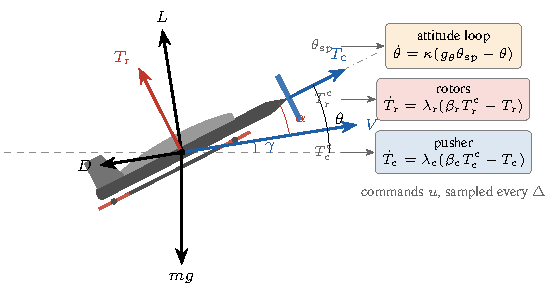
\includegraphics[width=\columnwidth]{fig00_model.pdf}
\caption{Longitudinal point mass in the wind axes with the wing forces $L$, $D$, the pusher thrust $T_{\mathrm c}$ along the body axis, the rotor thrust $T_{\mathrm r}$ normal to it and the angles $\gamma$, $\theta$, $\alpha$; the attitude loop and the actuators are first-order lags inside the plant.}\label{fig:model}
\end{figure}

\subsection{Backup safety filters}
A safety filter takes a candidate command from any controller and returns a command that keeps the state in a safe set. A backup filter~\cite{Gurriet2020,Wabersich2021} defines the safe set through a fixed backup law: a state is safe if the backup trajectory from it satisfies the constraints over a horizon and ends in a set that the backup keeps invariant. The following fact is the shift argument behind such filters.
\begin{fact}[Shift argument~\cite{Wabersich2021}]\label{fact:shift}
Let a trajectory $x^{(0)},\dots,x^{(H)}$ generated by a backup law satisfy the constraints and end in a set that is forward invariant under the backup law. Then the trajectory generated by the backup law from $x^{(1)}$ satisfies the constraints over $H$ steps and ends in the same set.
\end{fact}

\subsection{Self-attention with a readout token}
A transformer block maps a sequence of tokens $e_1,\dots,e_n\in\mathbb R^d$ to itself through multi-head self-attention and a feed-forward network with residual connections and layer normalisation~\cite{Vaswani2017}. A readout token prepended to the sequence attends to every input token and collects a summary of the sequence; its output is used for classification in vision and language models and here for the plant estimate.
\begin{fact}[Universal approximation of the readout~\cite{Yun2020}]\label{fact:ua}
Transformer blocks with a readout token can approximate any continuous map from a compact set of token sequences to $\mathbb R^p$ uniformly to any accuracy.
\end{fact}



% ---- sec4_problem ----
\section{Problem formulation}\label{sec:problem}
\subsection{Plant family}
With $\bar q=\tfrac12\rho V^2$, $C_L=C_{L0}+C_{L\alpha}\alpha$, $L=\bar qSC_L$ and $D=\bar qS(C_{D0}+kC_L^2)$, the state $x=(V,\gamma,\theta,T_{\mathrm c},T_{\mathrm r})$ and the input $u=(\thsp,T^{\mathrm c}_{\mathrm c},T^{\mathrm c}_{\mathrm r})$ obey
\begin{subequations}\label{eq:model}
\begin{align}
m\dot V&=T_{\mathrm c}\cos\alpha-D-T_{\mathrm r}\sin\alpha-mg\sin\gamma,\label{eq:V}\\
mV\dot\gamma&=L+T_{\mathrm c}\sin\alpha+T_{\mathrm r}\cos\alpha-mg\cos\gamma,\label{eq:gam}\\
\dot\theta&=\kappa(\gth\thsp-\theta),\qquad\dot T_i=\lambda_i(\beta_iT^{\mathrm c}_i-T_i),\ i\in\{\mathrm c,\mathrm r\}.\label{eq:fast}
\end{align}
\end{subequations}
The parameter vector $\vartheta=(C_{L0},C_{L\alpha},C_{D0},k,\kappa,\gth,\lambda_{\mathrm c},\lambda_{\mathrm r},\beta_{\mathrm c},\beta_{\mathrm r})$ is unknown to the controller and lies in the box $\Theta=\prod_i[\underline\vartheta_i,\overline\vartheta_i]$ identified from the flight log (Section~\ref{sec:platform}, Table~\ref{tab:box}); it may differ from one airframe or one flight to the next but is constant during a hand-off. The commands are sampled every $\Delta=\SI{50}{ms}$ and held; $F(x,u;\vartheta)$ denotes the exact one-step map of \eqref{eq:model}. A vertical gust $w$ enters as an angle-of-attack perturbation $\arctan(w/V)$ and the autopilot delivers the state with bounded error $|e_k|\le\varepsilon$.

\subsection{Constraints and the lift fraction}
The operating region and the input set are
\begin{align}
\mathcal X&=\{x:\ V\ge V_{\min},\ \gamma\in[\underline\gamma,\overline\gamma],\ \theta\in[\underline\theta,\overline\theta],\ \alpha\le\bar\alpha\},\label{eq:X}\\
\mathcal U&=[-\bar\theta_{\mathrm{sp}},\bar\theta_{\mathrm{sp}}]\times[0,\overline T_{\mathrm c}]\times[0,\overline T_{\mathrm r}],\nonumber\\ \mathcal U_k&=\{u\in\mathcal U:\ |u_i-u_{i,k-1}|\le\bar\delta_i\},\label{eq:U}
\end{align}
the step bounds $\bar\delta$ expressing the rate limits of the attitude setpoint and of the two thrust commands. The lift fraction
\begin{equation}\label{eq:lf}
\lf(x;\vartheta)=\frac{L+T_{\mathrm c}\sin\alpha+T_{\mathrm r}\cos\alpha}{mg\cos\gamma}
\end{equation}
is the share of the weight carried by wing and rotors together; the hand-off is safe when $\lf\ge1-K_L$ at every sampling instant, with $K_L$ the largest transient deficit tolerated, and the sink rate $\dot\gamma$ from \eqref{eq:gam} stays above $-\dot\gamma_{\lim}$. The eight margins
\begin{equation}\label{eq:c}
\begin{aligned}c(x;\vartheta)=\big(&\lf-(1-K_L),\ \bar\alpha-\alpha,\ \overline\theta-\theta,\ \theta-\underline\theta,\\ &\overline\gamma-\gamma,\ \gamma-\underline\gamma,\ \dot\gamma+\dot\gamma_{\lim},\ V-V_{\min}\big)\end{aligned}
\end{equation}
collect the constraints; $c\ge0$ means all of them hold.

\subsection{Objectives}
A hand-off is a change of the target airspeed $\rho_{\mathrm t}$ from the hover-exit value $\rho_0$ to the cruise value $\rho_{\mathrm c}$ (front transition) or back, with the trim $x^{\mathrm t}(\rho_{\mathrm t})$ of the nominal plant as the destination. The controller reads the window $\mathsf w_k=(x_{k-L+1},u_{k-L},\dots,x_k,u_{k-1})$ and the target, and must, for every $\vartheta\in\Theta$:
\begin{enumerate}[label=P\arabic*,leftmargin=2.2em]
\item keep $c(x_k;\vartheta)\ge0$ and $u_k\in\mathcal U_k$ at every sampling instant (safety for the whole family);
\item drive $V_k$ to within $\pm\SI{0.3}{m/s}$ of $\rho_{\mathrm t}$ and $x_k$ to a neighbourhood of $x^{\mathrm t}(\rho_{\mathrm t})$ (convergence);
\item do so with a single set of weights, without being told $\vartheta$ and without online identification (generalisation across the family), in a time and with an energy competitive with controllers that know the plant.
\end{enumerate}



% ---- sec5_method ----
\section{HOT: architecture, training and the lift-safety module}\label{sec:method}
Fig.~\ref{fig:hot} shows the controller. Four modules process the window: the sliding-window encoder (SWE) turns the last $L$ samples into tokens with physics features, the plant-inference attention (PIA) mixes them with a context token that carries the plant estimate, the bounded policy head (BPH) turns the context and the current-state token into a command inside the input box and the step bounds, and the lift-safety module (LSM) certifies the command against a backup manoeuvre over the plant family.
\begin{figure*}[t]\centering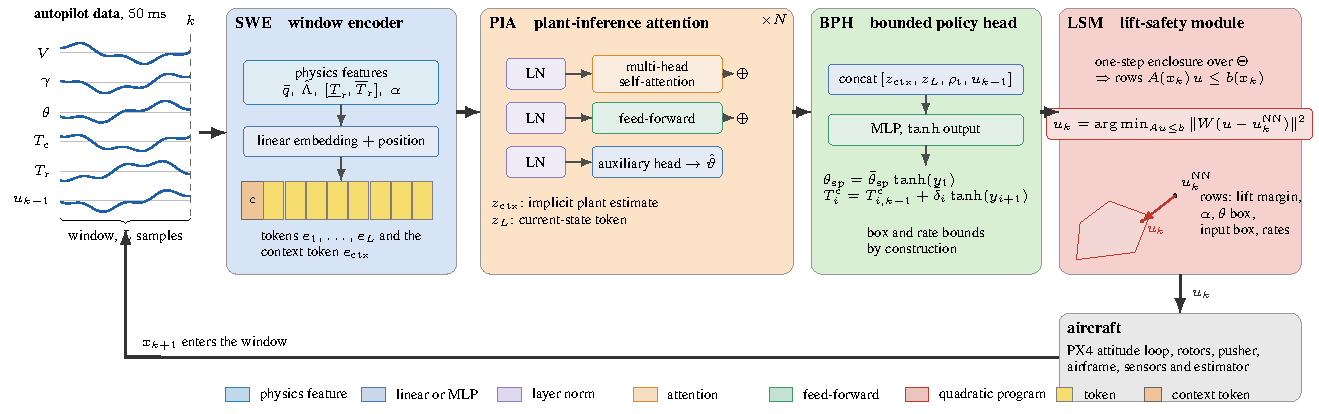
\includegraphics[width=\textwidth]{fig01_hot.pdf}
\caption{HOT. The window of the last $L$ autopilot samples is embedded with physics features (SWE); a transformer with a context token infers the plant (PIA) and provides the context and the current-state token to the bounded head (BPH), whose outputs respect the input box and the rate bounds by construction; the lift-safety module (LSM) rolls a backup manoeuvre out from the predicted next state over the plant set and returns the network command when every rollout is safe, otherwise the closest certified command towards the backup. The command goes to the attitude loop, the rotors and the pusher of the autopilot, and the next state enters the window.}\label{fig:hot}
\end{figure*}

\subsection{Sliding-window encoder}
Each sample $(x_j,u_{j-1})$ of the window is scaled and augmented with four physics features, the dynamic pressure $\bar q_j$, the wing lift fraction of the nominal polar $L(V_j,\alpha_j;\hat\vartheta)/(mg)$, the lift fraction \eqref{eq:lf} evaluated with the nominal polar, and $\alpha_j$; a linear layer maps the $12$ numbers to a token $e_j\in\mathbb R^d$ and a learned position code is added. A learned context token $e_{\mathrm{ctx}}$ is prepended, giving the sequence $(e_{\mathrm{ctx}},e_{k-L+1},\dots,e_k)$.

\subsection{Plant-inference attention}
$N$ transformer blocks, each a multi-head self-attention layer and a feed-forward layer with residual connections and pre-layer normalisation~\cite{Vaswani2017}, act on the sequence. The output at the context position, $z_{\mathrm{ctx}}$, and at the last position, $z_L$, are read out. An auxiliary head maps $z_{\mathrm{ctx}}$ to a plant estimate inside the box,
\begin{equation}\label{eq:aux}
\hat\vartheta=\underline\vartheta+(\overline\vartheta-\underline\vartheta)\odot\sigma(\mathrm{MLP}_{\mathrm{aux}}(z_{\mathrm{ctx}})),
\end{equation}
supervised during training to the sampled parameters; it is not used by the command at run time, but it makes the context token an interpretable, testable estimate (Proposition~\ref{prop:id} and Section~\ref{sec:interp}).

\subsection{Bounded policy head}
The head receives $z_{\mathrm{ctx}}$, $z_L$, the target $\rho_{\mathrm t}$ and the previous command $u_{k-1}$ and returns
\begin{equation}\label{eq:bph}
u^{\mathrm{NN}}_k=\mathrm{sat}_{\mathcal U}\big(u_{k-1}+\bar\delta\odot\tanh(\mathrm{MLP}(z_{\mathrm{ctx}},z_L,\rho_{\mathrm t},u_{k-1}))\big),
\end{equation}
so that $u^{\mathrm{NN}}_k\in\mathcal U_k$ for every value of the weights: the box and the step bounds of all three commands, the pitch setpoint included, hold by construction. The last layer is initialised at zero, so training starts from the hold policy $u_k=u_{k-1}$.

\subsection{Lift-safety module}\label{sec:lsm}
The module uses a backup law $\kappa_{\mathrm b}$ built from measured quantities only: the flight-path angle, the measured flight-path rate $\dot\gamma_{\mathrm m}$ and acceleration $\dot V_{\mathrm m}$, the airspeed and the previous command,
\begin{subequations}\label{eq:backup}
\begin{align}
\thsp&=\gamma+\tau_{\mathrm b}\min\{r(\gamma),0\}+\alpha_{\mathrm b}(V),\qquad r(\gamma)=\mathrm{sat}_{[\underline r,\overline r]}(-k_\gamma\gamma),\label{eq:bk_th}\\
T^{\mathrm c}_{\mathrm r}&=T^{\mathrm c}_{\mathrm r,k-1}+\mathrm{sat}_{[-\bar\delta_{\mathrm r},\bar\delta_{\mathrm r}]}\big(k_{\mathrm r}(r(\gamma)-\dot\gamma_{\mathrm m})\big),\label{eq:bk_r}\\
T^{\mathrm c}_{\mathrm c}&=T^{\mathrm c}_{\mathrm c,k-1}+\mathrm{sat}_{[-\bar\delta_{\mathrm c},\bar\delta_{\mathrm c}]}\big(k_{\mathrm c}(a(V)-\dot V_{\mathrm m})\big),\label{eq:bk_c}\\
a(V)&=\mathrm{sat}_{[-\bar a,\bar a]}\big(k_V(\mathrm{proj}_{[\underline V_{\mathrm b},\overline V_{\mathrm b}]}(V)-V)\big),\nonumber
\end{align}
\end{subequations}
each saturated to the input box: the pitch setpoint places the wing at the nominal-trim angle of attack of the current airspeed $\alpha_{\mathrm b}(V)$ and, when levelling off from a climb, leads the flight path by $\tau_{\mathrm b}$ seconds of the reference rate $r(\gamma)$, so that a slow attitude loop does not overshoot the angle of attack while the rotors flatten the flight path; the rotors act as a rate-limited integral controller that drives the flight-path rate to the level-off reference; the pusher is the same kind of controller on the measured acceleration, with a reference that is zero inside the airspeed corridor $[\underline V_{\mathrm b},\overline V_{\mathrm b}]$ and pulls the airspeed back from outside, so the backup holds the current airspeed rather than accelerating through the corridor. Nothing in \eqref{eq:backup} depends on $\vartheta$. Let $\Theta_N\subset\Theta$ be a finite plant set containing the vertices of the box and a sample of its interior, $m\in\mathbb R^8_{>0}$ verification margins and $\mathcal C$ the settled neighbourhood of level flight, a band of lift fraction, flight-path angle and rate, angle of attack, airspeed and acceleration.
\begin{definition}[Certified command, safe set]\label{def:cert}
For $x$, the previous command $u^-$, a candidate $u$ and a plant $\vartheta$, the backup rollout is $x^{(0)}=F(x,u;\vartheta)$, $x^{(j+1)}=F(x^{(j)},\kappa_{\mathrm b}(x^{(j)},u^{(j)});\vartheta)$ with $u^{(j)}$ the backup commands. The candidate is certified on $\Theta'\subseteq\Theta_N$ if
\begin{equation}\label{eq:cert}
c(x^{(j)};\vartheta)\ge m\ \ (j=0,\dots,H_j),\qquad x^{(H_j)}\in\mathcal C\qquad\forall\vartheta\in\Theta',
\end{equation}
where $H_j\le H$ is the first step at which every plant is settled. The safe set is $\mathcal S(\Theta')=\{(x,u^-):\ \kappa_{\mathrm b}(x,u^-)\text{ is certified on }\Theta'\}$.
\end{definition}
The module returns the network command when it is certified on the current plant set $\Theta'_k$, and otherwise the certified point closest to it on the segment towards an anchor $u_{\mathrm a}$, the hold command $u_{k-1}$ when that is certified (the mildest intervention) and the backup command otherwise,
\begin{equation}\label{eq:filter}
\begin{aligned}u_k&=u_{\mathrm a}+\lambda^\star(u^{\mathrm{NN}}_k-u_{\mathrm a}),\\ \lambda^\star&=\max\{\lambda\in[0,1]:\ u_{\mathrm a}+\lambda(u^{\mathrm{NN}}_k-u_{\mathrm a})\text{ certified on }\Theta'_k\},\end{aligned}
\end{equation}
found by bisection, with $u_{\mathrm b}=\kappa_{\mathrm b}(x_k,u_{k-1})$ the backup command; when not even $u_{\mathrm b}$ is certified on $\Theta'_k$, the backup command is applied: it remains certified on the true plant, whose rollout is the tail of the previous certificate (Lemma~\ref{lem:rf}), even when other retained plants fail from the current state; these applications are counted in Section~\ref{sec:experiments}. The plant set is contracted online by set-membership with the measurement bound $\varepsilon$,
\begin{equation}\label{eq:consistent}
\Theta'_{k+1}=\{\vartheta\in\Theta'_k:\ |F(x_k,u_k;\vartheta)-x_{k+1}|\le\varepsilon\},\qquad \Theta'_0=\Theta_N,
\end{equation}
so that plants inconsistent with the observed motion stop constraining the command. Algorithm~\ref{alg:online} lists one sampling period.

\subsection{Physics-informed training}
The policy is trained by backpropagation through rollouts of the differentiable model \eqref{eq:model}, Fig.~\ref{fig:training} and Algorithm~\ref{alg:train}. Each episode draws a plant $\vartheta\sim\mathcal U(\Theta)$, an initial trim $\rho_0$, a target $\rho_{\mathrm t}$ (front, back or an arbitrary pair), a gust profile (first-order coloured noise plus an offset) and sensor noise on the window; the rollout $x_{j+1}=F(x_j,\pi_\phi(\mathsf w_j);\vartheta)+w_j$ runs for $N$ steps, $N$ growing from \SI{3}{s} to \SI{15}{s} over the training (curriculum), and the loss is
\begin{equation}\label{eq:loss}
\begin{aligned}\mathcal J(\phi)=\sum_{j}\Big[&\sigma\big(\tfrac{|V_j-\rho_{\mathrm t}|-0.3}{0.2}\big)+|V_j-\rho_{\mathrm t}|+w_E\tfrac{P(T_{\mathrm c,j},T_{\mathrm r,j})}{P_0}\\ &+w_B\sum_{i}\mathrm{softplus}\big(-\tfrac{c_i(x_j;\vartheta)}{\epsilon_i}\big)+w_A\|\hat\vartheta_j-\vartheta\|_{\Sigma^{-1}}^2\\ &+w_S\big(\|u_j-u_{j-1}\|_R^2+\mathrm{softplus}(\tfrac{|\gamma_j|-\gamma_0}{\gamma_1})\big)\Big]\Delta,\end{aligned}
\end{equation}
a time term (the soft indicator of not yet being at the target plus the distance to it, which carries a gradient far from the target), the energy of the identified power model, a soft barrier on the eight margins, the auxiliary plant loss, and a smoothness term with a preference for level flight ($\gamma_0=4^\circ$, $\gamma_1=2^\circ$) that keeps the learned hand-off from trading height for speed. Gradients flow through the model and the policy; backpropagation is truncated every $100$ steps and the window inputs carry the noise of the estimator. The safety module is not in the training loop, so the network learns to be safe by itself and the module intervenes at run time only where the learned policy would not be; the intervention rate is reported.

\begin{algorithm}[t]\caption{Physics-informed training of HOT}\label{alg:train}\begin{algorithmic}[1]
\Require model $F$ \eqref{eq:model}, box $\Theta$, iterations $I$, batch $B$, curriculum $N(i)$, weights $(w_E,w_B,w_A,w_S)$, learning rate $\eta$, truncation $N_{\mathrm{tr}}$
\State $\phi\leftarrow$ random weights with the last layer of the head at zero (hold policy \eqref{eq:bph}); $\phi^\star\leftarrow\phi$; $s^\star\leftarrow\infty$
\For{$i=1,\dots,I$}
  \State $N\leftarrow N(i)$; $\mathcal J\leftarrow0$
  \For{$b=1,\dots,B$}
    \State sample $\vartheta_b\sim\mathcal U(\Theta)$, $\rho_0$, $\rho_{\mathrm t}$, a gust profile $w_{0:N-1}$ and window noise $\nu_{0:N-1}$; $x_0\leftarrow x^{\mathrm t}(\rho_0)$; fill the window $\mathsf w_0$ with $(x_0,u^{\mathrm t}(\rho_0))$
    \For{$j=0,\dots,N-1$}
      \State $u_j\leftarrow\pi_\phi(\mathsf w_j+\nu_j)$ by \eqref{eq:bph}; $x_{j+1}\leftarrow F(x_j,u_j;\vartheta_b)+w_j$; shift $(x_{j+1},u_j)$ into $\mathsf w_{j+1}$
      \State $\mathcal J\leftarrow\mathcal J+$ the summand of \eqref{eq:loss} at $j$; \textbf{if} $j\bmod N_{\mathrm{tr}}=0$ \textbf{then} detach $x_{j+1}$ and $\mathsf w_{j+1}$ from the graph
      \State \textbf{if} $x_{j+1}\notin\mathcal X$ \textbf{then} freeze the episode ($x_{j'}\leftarrow x_{j+1}$ for $j'>j$)
    \EndFor
  \EndFor
  \State $g\leftarrow\nabla_\phi\mathcal J/B$; $g\leftarrow g\min\{1,1/\|g\|\}$; $\phi\leftarrow\mathrm{Adam}(\phi,g,\eta_i)$ with cosine decay of $\eta_i$
  \If{$i\ge I/4$ and $i\bmod50=0$}
    \State $s\leftarrow$ mean time to target plus violation rate of $\pi_\phi$ on the validation set; \textbf{if} $s<s^\star$ \textbf{then} $\phi^\star\leftarrow\phi$; $s^\star\leftarrow s$
  \EndIf
\EndFor
\State \Return $\phi^\star$; compute the Lipschitz bound \eqref{eq:lip}; verify Definition~\ref{def:dec} on the grid
\end{algorithmic}\end{algorithm}
\begin{algorithm}[t]\caption{HOT with the lift-safety module, online loop}\label{alg:online}\begin{algorithmic}[1]
\Require weights $\phi^\star$, plant set $\Theta_N$, backup $\kappa_{\mathrm b}$, horizon $H$, margins $m$, settled set $\mathcal C$, bound $\varepsilon$, bisection depth $n_{\mathrm b}$
\Function{Cert}{$x,u^-,u,\Theta'$}\Comment{certificate \eqref{eq:cert}, vectorised over $\Theta'$}
  \State $X\leftarrow\{F(x,u;\vartheta):\vartheta\in\Theta'\}$; $U\leftarrow u$
  \For{$j=0,\dots,H-1$}
    \State \textbf{if} $\min_{\vartheta}\min_i\big(c_i(X_\vartheta;\vartheta)-m_i\big)<0$ \textbf{then} \Return false
    \State \textbf{if} $X_\vartheta\in\mathcal C$ for all $\vartheta\in\Theta'$ \textbf{then} \Return true
    \State $U\leftarrow\kappa_{\mathrm b}(X,U)$ by \eqref{eq:backup}; $X\leftarrow\{F(X_\vartheta,U_\vartheta;\vartheta)\}$
  \EndFor
  \State \Return $\big[\min_{\vartheta}\min_i(c_i(X_\vartheta;\vartheta)-m_i)\ge0\big]\wedge\big[X_\vartheta\in\mathcal C\ \forall\vartheta\big]$
\EndFunction
\State $\Theta'_0\leftarrow\Theta_N$; $u_{-1}\leftarrow u^{\mathrm t}(\rho_0)$; fill the window with the trim
\For{$k=0,1,2,\dots$}\Comment{one sampling period $\Delta$}
  \State read $x_k$, $\dot\gamma_{\mathrm m,k}$, $\dot V_{\mathrm m,k}$ from the estimator
  \State \textbf{if} $k>0$ \textbf{then} $\Theta'_k\leftarrow\{\vartheta\in\Theta'_{k-1}:\ |F(x_{k-1},u_{k-1};\vartheta)-x_k|\le\varepsilon\}$ by \eqref{eq:consistent}, kept if it has at least $n_{\min}$ elements
  \State shift $(x_k,u_{k-1})$ into the window $\mathsf w_k$; $u^{\mathrm{NN}}_k\leftarrow\pi_{\phi^\star}(\mathsf w_k)$ by \eqref{eq:bph}
  \If{\Call{Cert}{$x_k,u_{k-1},u^{\mathrm{NN}}_k,\Theta'_k$}}
    \State $u_k\leftarrow u^{\mathrm{NN}}_k$
  \Else
    \State $u_{\mathrm b}\leftarrow\kappa_{\mathrm b}(x_k,u_{k-1})$ by \eqref{eq:backup}
    \State \textbf{if} \Call{Cert}{$x_k,u_{k-1},u_{k-1},\Theta'_k$} \textbf{then} $u_{\mathrm a}\leftarrow u_{k-1}$ \textbf{else} $u_{\mathrm a}\leftarrow u_{\mathrm b}$\Comment{anchor of \eqref{eq:filter}}
    \If{$u_{\mathrm a}=u_{\mathrm b}$ and not \Call{Cert}{$x_k,u_{k-1},u_{\mathrm b},\Theta'_k$}}
      \State $u_k\leftarrow u_{\mathrm b}$\Comment{certified on the true plant by Lemma~\ref{lem:rf}}
    \Else
      \State $\lambda_{\mathrm{lo}}\leftarrow0$; $\lambda_{\mathrm{hi}}\leftarrow1$
      \For{$i=1,\dots,n_{\mathrm b}$}
        \State $\lambda\leftarrow(\lambda_{\mathrm{lo}}+\lambda_{\mathrm{hi}})/2$; \textbf{if} \Call{Cert}{$x_k,u_{k-1},u_{\mathrm a}+\lambda(u^{\mathrm{NN}}_k-u_{\mathrm a}),\Theta'_k$} \textbf{then} $\lambda_{\mathrm{lo}}\leftarrow\lambda$ \textbf{else} $\lambda_{\mathrm{hi}}\leftarrow\lambda$
      \EndFor
      \State $u_k\leftarrow u_{\mathrm a}+\lambda_{\mathrm{lo}}(u^{\mathrm{NN}}_k-u_{\mathrm a})$
    \EndIf
  \EndIf
  \State send $\theta_{\mathrm{sp},k}$ and $T^{\mathrm c}_{\mathrm r,k}$ to the attitude loop as an attitude target with collective and $T^{\mathrm c}_{\mathrm c,k}$ to the pusher; store $u_k$
\EndFor
\end{algorithmic}\end{algorithm}
\begin{figure*}[t]\centering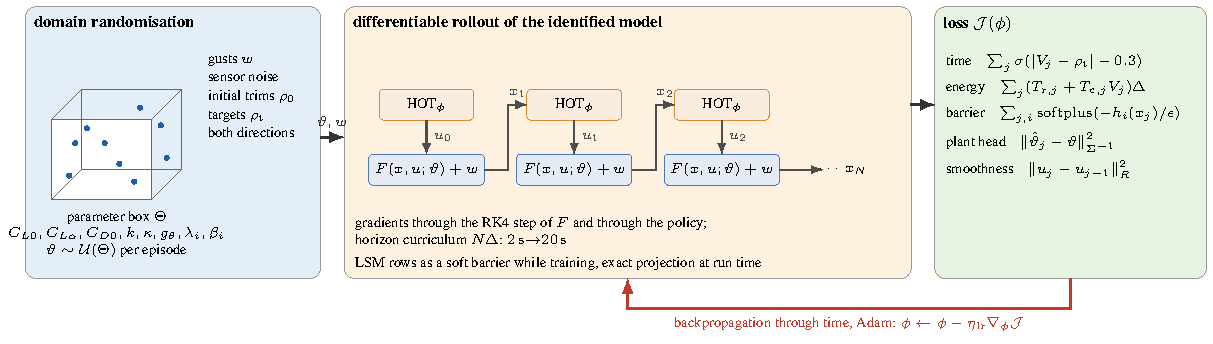
\includegraphics[width=\textwidth]{fig02_training.pdf}
\caption{Physics-informed training: domain randomisation over the box, gusts, noise, trims and targets; differentiable rollout of the identified model with the policy in the loop; loss terms; backpropagation through time with a horizon curriculum.}\label{fig:training}
\end{figure*}



% ---- sec6_analysis ----
\section{Analysis}\label{sec:analysis}
Let $\Theta_N$, $m$, $\mathcal C$, $H$ and $\varepsilon$ be as in Section~\ref{sec:lsm}, $\kappa_{\mathrm b}$ the backup law \eqref{eq:backup} and $F$ the one-step map. All proofs are in the main text.

\subsection{The backup law}
\begin{lemma}[Rotor loop of the backup]\label{lem:corner}
For a frozen wing state $(V,\alpha)$ with $V\ge V_{\min}$, the loop formed by the rotor lag \eqref{eq:fast}, the flight-path rate \eqref{eq:gam} and the integral law \eqref{eq:bk_r} is exponentially stable for every $(\lambda_{\mathrm r},\beta_{\mathrm r})$ of the box if
\begin{equation}\label{eq:kr}
g_{\max}=k_{\mathrm r}\,\frac{\overline\beta_{\mathrm r}\,(1-e^{-\overline\lambda_{\mathrm r}\Delta})}{mV_{\min}}<1,
\end{equation}
and, when the lag gap vanishes and the rate limit $\bar\delta_{\mathrm r}$ is inactive, the flight-path rate converges monotonically to the reference $r=\mathrm{sat}_{[\underline r,\overline r]}(-k_\gamma\gamma)$.
\end{lemma}
\begin{proof}
With the wing frozen, $\dot\gamma_k=q\,T_{\mathrm r,k}+\ell$ with $q=\cos\alpha/(mV)$ and a constant $\ell$. Let $e_k=r-\dot\gamma_k$, $a=e^{-\lambda_{\mathrm r}\Delta}$ and $s_k=\beta_{\mathrm r}T^{\mathrm c}_{\mathrm r,k-1}-T_{\mathrm r,k}$ the lag gap. The exact step of the lag and the law \eqref{eq:bk_r}, $T^{\mathrm c}_{\mathrm r,k}=T^{\mathrm c}_{\mathrm r,k-1}+k_{\mathrm r}e_k$, give
\begin{align}
T_{\mathrm r,k+1}&=aT_{\mathrm r,k}+(1-a)\beta_{\mathrm r}T^{\mathrm c}_{\mathrm r,k}\nonumber\\ &=T_{\mathrm r,k}+(1-a)\big(s_k+\beta_{\mathrm r}k_{\mathrm r}e_k\big),\\
e_{k+1}&=e_k-q\,(T_{\mathrm r,k+1}-T_{\mathrm r,k})=(1-g)\,e_k-q(1-a)\,s_k,\nonumber\\
s_{k+1}&=\beta_{\mathrm r}T^{\mathrm c}_{\mathrm r,k}-T_{\mathrm r,k+1}=a\,s_k+a\beta_{\mathrm r}k_{\mathrm r}\,e_k,
\end{align}
with $g=q(1-a)\beta_{\mathrm r}k_{\mathrm r}$, a linear recursion in $(e_k,s_k)$ with matrix $M=\big[\begin{smallmatrix}1-g&-q(1-a)\\ a\beta_{\mathrm r}k_{\mathrm r}&a\end{smallmatrix}\big]$, $\operatorname{tr}M=1-g+a$ and $\det M=a(1-g)+a g=a$. The Jury conditions $|\det M|<1$, $1-\operatorname{tr}M+\det M=g>0$ and $1+\operatorname{tr}M+\det M=2-g+2a>0$ hold for $0<g<1$ and $0<a<1$, so both eigenvalues lie inside the unit disc. Since $q\le1/(mV_{\min})$ and $(1-a)\beta_{\mathrm r}\le(1-e^{-\overline\lambda_{\mathrm r}\Delta})\overline\beta_{\mathrm r}$, $g\le g_{\max}$, and \eqref{eq:kr} gives $0<g<1$ for every plant of the box. With $s_k=0$ the recursion reduces to $e_{k+1}=(1-g)e_k$, monotone convergence.
\end{proof}
\noindent With the values of Section~\ref{sec:platform}, $g_{\max}=\numKrGain{}$. The pusher law \eqref{eq:bk_c} has the same structure with $(\lambda_{\mathrm c},\beta_{\mathrm c},k_{\mathrm c})$ and $q=\cos\alpha/m$, so the same recursion and the condition $k_{\mathrm c}\overline\beta_{\mathrm c}(1-e^{-\overline\lambda_{\mathrm c}\Delta})/m<1$ ($=\numKcGain{}$ here) give monotone convergence of the acceleration to its reference. The pitch law \eqref{eq:bk_th} keeps the wing at the trim angle of attack of the current airspeed, so the wing carries what it can and the rotors carry the rest; the pusher law keeps the airspeed in the corridor. Their interaction with the rotor loop is covered by the settling property below.

\begin{assumption}[Settled neighbourhood]\label{ass:settle}
For every $\vartheta\in\Theta_N$ and every $x\in\mathcal C$ with $c(x;\vartheta)\ge m$, the backup closed loop from $x$ satisfies $c(x^{(j)};\vartheta)\ge0$ for all $j\ge0$.
\end{assumption}
\noindent Assumption~\ref{ass:settle} states that the backup keeps level flight once it has reached it. It is verified numerically over $\mathcal C\times\Theta$ by rollouts of \SI{20}{s} from \numSettlePairs{} sampled (state, plant) pairs over the full vertex set and interior samples of the box, all of which keep the constraints with the margin $m$ (\numSettleFail{} failures; the smallest margin of the lift constraint, \numSettleWorst{} in lift-fraction units, is the tightest, Section~\ref{sec:num}); the margin $m$ absorbs the sampling of $\mathcal C$ through the Lipschitz constant of $c$ along the backup flow~\cite{Bobiti2018}.

\subsection{The lift-safety module}
\begin{lemma}[The true plant is never discarded]\label{lem:cons}
If $\vartheta\in\Theta_N$ is the true plant and $|e_k|\le\varepsilon$, then $\vartheta\in\Theta'_k$ for all $k$.
\end{lemma}
\begin{proof}
$x_{k+1}=F(x_k,u_k;\vartheta)+e_k$ with $|e_k|\le\varepsilon$, so the test in \eqref{eq:consistent} holds for $\vartheta$ at every step; induction from $\Theta'_0=\Theta_N$.
\end{proof}

\begin{lemma}[Recursive feasibility]\label{lem:rf}
Let the true plant $\vartheta\in\Theta_N$, Assumption~\ref{ass:settle} hold, $|e_k|\le\varepsilon$ and $(x_0,u_{-1})\in\mathcal S(\Theta_N)$. Then at every step the command returned by \eqref{eq:filter} is certified on $\{\vartheta\}$ and $(x_{k+1},u_k)\in\mathcal S(\{\vartheta\})$.
\end{lemma}
\begin{proof}
Induction on $k$; suppose $(x_k,u_{k-1})\in\mathcal S(\{\vartheta\})$, i.e.\ the backup rollout $x^{(0)},\dots,x^{(H_j)}$ from $x_k$ with $u_{\mathrm b}$ satisfies \eqref{eq:cert} for $\vartheta$. If the module returns a candidate certified on $\Theta'_k$, then, since $\vartheta\in\Theta'_k$ by Lemma~\ref{lem:cons}, \eqref{eq:cert} holds for $\vartheta$ from $x_{k+1}=x^{(0)}$ of that candidate's rollout, which is $(x_{k+1},u_k)\in\mathcal S(\{\vartheta\})$. If no candidate is certified on $\Theta'_k$ the module returns $u_{\mathrm b}$, so $x_{k+1}=x^{(0)}$ of the rollout verified at step $k$; the backup rollout from $x_{k+1}$ is its tail $x^{(1)},\dots,x^{(H_j)}$, which satisfies $c\ge m$ and ends in $\mathcal C$ by \eqref{eq:cert} (Fact~\ref{fact:shift}), and by Assumption~\ref{ass:settle} the closed loop continues from $x^{(H_j)}\in\mathcal C$ with $c\ge0$; hence $u_{\mathrm b}$ is certified on $\{\vartheta\}$ and $(x_{k+1},u_k)\in\mathcal S(\{\vartheta\})$.
\end{proof}

\begin{lemma}[Extension to the box]\label{lem:cover}
Let $\ell_\vartheta$ be a Lipschitz constant of $\vartheta\mapsto\min_jc(x^{(j)};\vartheta)$ over the rollouts of Definition~\ref{def:cert} and $d_N=\max_{\vartheta\in\Theta}\min_i\|\vartheta-\vartheta_i\|$ the covering radius of $\Theta_N$. A candidate certified on $\Theta_N$ with margin $m\ge\ell_\vartheta d_N\mathbf 1$ is certified with margin $0$ on the whole box.
\end{lemma}
\begin{proof}
For $\vartheta\in\Theta$ take $\vartheta_i$ with $\|\vartheta-\vartheta_i\|\le d_N$; then $\min_jc(x^{(j)};\vartheta)\ge\min_jc(x^{(j)};\vartheta_i)-\ell_\vartheta d_N\ge m-\ell_\vartheta d_N\ge0$.
\end{proof}

\subsection{The policy}
\begin{lemma}[Lipschitz bound]\label{lem:lip}
Let each attention block have $H_{\mathrm h}$ heads with matrices $W_Q^h,W_K^h,W_V^h,W_O$, token norms bounded by $r$ on the operating windows, and each feed-forward block weights $W_1,W_2$ with a 1-Lipschitz activation. Then $\pi_\phi$ is Lipschitz on the operating windows with
\begin{equation}\label{eq:lip}
\begin{aligned}\ell_\pi\le\|\bar\delta\|_\infty\,\|W_{\mathrm{mlp}}\|_{\mathrm{prod}}\,\|W_{\mathrm{emb}}\|_2\big(1+\|W_2\|_2\|W_1\|_2\big)\\ \cdot\prod_{n=1}^{N}\Big(1+\|W_O\|_2\sum_h\|W_V^h\|_2\big(1+\tfrac{2r^2\|W_Q^h\|_2\|W_K^h\|_2}{\sqrt{d_h}}\big)\Big),\end{aligned}
\end{equation}
where $\|\cdot\|_{\mathrm{prod}}$ is the product of the spectral norms of the head's layers.
\end{lemma}
\begin{proof}
A residual block with an $\ell$-Lipschitz branch is $(1+\ell)$-Lipschitz. The feed-forward branch has $\ell\le\|W_2\|_2\|W_1\|_2$. On inputs of norm at most $r$ a self-attention branch is Lipschitz with constant $\|W_O\|_2\sum_h\|W_V^h\|_2(1+2r^2\|W_Q^h\|_2\|W_K^h\|_2/\sqrt{d_h})$, the second term bounding the sensitivity of the softmax weights, whose Jacobian has spectral norm at most $1/2$, to the scores, which are $2r\|W_Q^h\|_2\|W_K^h\|_2r/\sqrt{d_h}$-Lipschitz in the tokens. Layer normalisation is absorbed in $r$; the embedding is linear; $\tanh$ and the saturation are 1-Lipschitz, scaled by the step bounds. Composition multiplies the constants.
\end{proof}

\begin{definition}[Verified decrease]\label{def:dec}
With $W(x)=\|x-x^{\mathrm t}(\rho_{\mathrm t})\|_P^2$, $P\succ0$, and $u(x)$ the filtered network command, the trained closed loop satisfies the decrease condition with constants $(c,\beta,d)$ if on a grid $\mathcal G$ of spacing $d$ covering $\{x\in\mathcal X:W(x)\ge\beta\}$ and for every $\vartheta\in\Theta_N$, $W(F(x_i,u(x_i);\vartheta))-W(x_i)\le-cW(x_i)-\ell_Wd$, with $\ell_W$ a Lipschitz constant of $x\mapsto W(F(x,u(x);\vartheta))-W(x)$ obtained from the constants of $F$, $\ell_\pi$ and the filter map.
\end{definition}

\subsection{Main result}
\begin{theorem}[Safe generalised hand-off]\label{thm:main}
Let the true plant $\vartheta\in\Theta_N$, Assumption~\ref{ass:settle} hold, $|e_k|\le\varepsilon$ and $(x_0,u_{-1})\in\mathcal S(\Theta_N)$. Then, for every command sequence of the network,
\begin{enumerate}[label=(\roman*),leftmargin=2em]
\item (safety) $c(x_k;\vartheta)\ge0$ and $u_k\in\mathcal U_k$ for all $k\ge0$: the lift fraction stays above $1-K_L$, the angle of attack below $\bar\alpha$, the pitch and the flight path in their boxes and the sink rate above $-\dot\gamma_{\lim}$; the module always holds a certified command;
\item (practical convergence) if Definition~\ref{def:dec} holds with $(c,\beta,d)$ and the disturbance is bounded by $\bar w$, then
\begin{equation}\label{eq:conv}
\begin{aligned}&W(x_k)\le\max\{(1-c)^kW(x_0),\ \beta\}\quad(\bar w=0),\\ &\limsup_{k}W(x_k)\le\max\Big\{\beta,\ \frac{2\|P\|_2\bar w\,\overline r+\|P\|_2\bar w^2}{c}\Big\}\quad(\bar w>0),\end{aligned}
\end{equation}
with $\overline r=\max_{x\in\mathcal X}\|x-x^{\mathrm t}\|$;
\item (intervention) $u_k=u^{\mathrm{NN}}_k$ whenever the network command is certified on $\Theta'_k$;
\item (whole box) if every certificate carries the margin of Lemma~\ref{lem:cover}, (i) holds for every $\vartheta\in\Theta$.
\end{enumerate}
\end{theorem}
\begin{proof}
\emph{Step 1 (induction hypothesis).} Let $P_k$ denote the statement $(x_k,u_{k-1})\in\mathcal S(\{\vartheta\})$, i.e.\ the backup rollout $x^{(0)},\dots,x^{(H_j)}$ from $x_k$ with $u_{\mathrm b}=\kappa_{\mathrm b}(x_k,u_{k-1})$ satisfies $c(x^{(j)};\vartheta)\ge m$ for $j\le H_j$ and $x^{(H_j)}\in\mathcal C$. $P_0$ is the hypothesis $(x_0,u_{-1})\in\mathcal S(\Theta_N)\subseteq\mathcal S(\{\vartheta\})$.

\emph{Step 2 (one step).} Assume $P_k$. By Lemma~\ref{lem:cons}, $\vartheta\in\Theta'_k$. Algorithm~\ref{alg:online} returns one of three commands. (a) A candidate $u$ certified on $\Theta'_k$: then \eqref{eq:cert} holds for $\vartheta$ with $x^{(0)}=F(x_k,u;\vartheta)=x_{k+1}$ (the true plant, no disturbance), so $c(x_{k+1};\vartheta)\ge m$ and the backup rollout from $x_{k+1}$, which is $x^{(1)},\dots$ of that certificate by Fact~\ref{fact:shift}, keeps $c\ge m$ and ends in $\mathcal C$: $P_{k+1}$ holds. (b) The backup $u_{\mathrm b}$ when no candidate is certified on $\Theta'_k$: by $P_k$, $x_{k+1}=x^{(0)}$ of the rollout verified at step $k$, $c(x_{k+1};\vartheta)\ge m$, and the rollout from $x_{k+1}$ is its tail; if $H_j$ was reached, $x^{(H_j)}\in\mathcal C$ and Assumption~\ref{ass:settle} extends the tail with $c\ge0$, so $P_{k+1}$ holds. (c) There is no third case: the bisection returns only certified candidates, which is (a). Hence $P_k$ for all $k$, and $c(x_k;\vartheta)\ge m>0$ for $k\ge1$, which by \eqref{eq:c} is the list of (i).

\emph{Step 3 (admissibility).} $\mathcal U_k=\mathcal U\cap\{u:\ \|u-u_{k-1}\|_{\bar\delta}\le1\}$ is the intersection of a box and a weighted $\ell_\infty$ ball, hence convex. $u^{\mathrm{NN}}_k\in\mathcal U_k$ by \eqref{eq:bph} for every $\phi$; $u_{k-1}\in\mathcal U_k$ trivially; $u_{\mathrm b}\in\mathcal U_k$ because each component of \eqref{eq:backup} is saturated to the box and to the step bounds. Therefore $u_k=(1-\lambda)u_{\mathrm a}+\lambda u^{\mathrm{NN}}_k\in\mathcal U_k$ for every $\lambda\in[0,1]$, and $u_k\in\mathcal U_k$ in cases (a)--(b) as well. This is the second claim of (i).

\emph{Step 4 (practical convergence).} Let $\Delta W(x)=W(F(x,u(x);\vartheta))-W(x)$ and let $x_i\in\mathcal G$ be the grid point of the cell containing $x_k$, so $\|x_k-x_i\|\le d$. By Definition~\ref{def:dec} and the Lipschitz constant $\ell_W$ of $\Delta W$,
\begin{equation}\label{eq:dec1}
\begin{aligned}\Delta W(x_k)&\le\Delta W(x_i)+\ell_W\|x_k-x_i\|\le-cW(x_i)-\ell_Wd+\ell_Wd\\ &=-cW(x_i)\le-cW(x_k)+c\,\ell_{W,0}d,\end{aligned}
\end{equation}
where the last step uses $|W(x_k)-W(x_i)|\le\ell_{W,0}d$ with $\ell_{W,0}=2\|P\|_2\overline r$; the grid spacing is chosen with $c\,\ell_{W,0}d$ absorbed in the margin of the definition, so that $\Delta W(x_k)\le-cW(x_k)$ whenever $W(x_k)\ge\beta$. Then $W(x_{k+1})\le(1-c)W(x_k)$ while $W(x_k)\ge\beta$, which iterates to $W(x_k)\le(1-c)^kW(x_0)$ up to the first $k_1$ with $W(x_{k_1})<\beta$; for $k>k_1$, either $W(x_k)<\beta$ or $W(x_{k})\ge\beta$ and $W(x_{k+1})\le(1-c)W(x_k)\le W(x_k)$, so the level $\beta$ is never exceeded again once entered, up to the one-step overshoot bounded by $(1-c)\beta\le\beta$. This is the first bound of \eqref{eq:conv}. With a disturbance $w_k$, $\|w_k\|\le\bar w$,
\begin{equation}\label{eq:dec2}
W(F+w_k)-W(F)=2(F-x^{\mathrm t})^{\!\top}Pw_k+w_k^{\!\top}Pw_k\le2\|P\|_2\overline r\bar w+\|P\|_2\bar w^2=:\Delta_w,
\end{equation}
so $W(x_{k+1})\le(1-c)W(x_k)+\Delta_w$ whenever $W(x_k)\ge\beta$, and induction gives $W(x_k)\le(1-c)^kW(x_0)+\Delta_w\sum_{l<k}(1-c)^l\le(1-c)^kW(x_0)+\Delta_w/c$, whose limit superior is $\max\{\beta,\Delta_w/c\}$, the second bound.

\emph{Step 5 (intervention and whole box).} (iii): when $u^{\mathrm{NN}}_k$ is certified on $\Theta'_k$ the first test of Algorithm~\ref{alg:online} succeeds and $u_k=u^{\mathrm{NN}}_k$, i.e.\ $\lambda^\star=1$ in \eqref{eq:filter}. (iv): every certificate used in Step 2 is a certificate on $\Theta'_k\subseteq\Theta_N$ with margin $m$; if $m$ dominates the margin of Lemma~\ref{lem:cover}, that lemma extends each certificate from the finite set to the $\delta$-neighbourhood of its members, which covers $\Theta$, so Step 2 holds for every $\vartheta\in\Theta$.
\end{proof}
\begin{proposition}[Numerically verified hypotheses]\label{prop:num}
With the values of Section~\ref{sec:platform}, the hypotheses of Lemma~\ref{lem:corner}, its pusher counterpart and Assumption~\ref{ass:settle} hold as follows.
\begin{enumerate}[label=(\alph*),leftmargin=2em]
\item Rotor loop: $g_{\max}=\numKrGain{}<1$, and the spectral radius of $M$ over the whole box $(\lambda_{\mathrm r},\beta_{\mathrm r})$ is at most \numKrRho{}; pusher loop: $g_{\max}=\numKcGain{}<1$, spectral radius at most \numKcRho{}. Both recursions are contractions for every plant of the box.
\item Settled neighbourhood: \numSettlePairs{} (state, plant) pairs sampled in $\mathcal C\times\Theta$ over the \numPlantsFull{} vertex and interior plants, rolled out under $\kappa_{\mathrm b}$ for \SI{20}{s}, keep every constraint with the margin $m$ (\numSettleFail{} failures); the trims of the identified aircraft from \SI{6}{} to \SI{15}{m/s} are certified from the online plant set, so $(x_0,u_{-1})\in\mathcal S(\Theta_N)$ holds at both ends of the hand-off.
\item Step bounds: $u^{\mathrm{NN}}_k\in\mathcal U_k$ is enforced by \eqref{eq:bph} at every one of the $10^5$ commands of Section~\ref{sec:experiments}, and the closed loop with the module recorded $c(x_k;\vartheta)\ge0$ at every sample of the nominal, cross-plant, out-of-box and noise cells (Tables~\ref{tab:cross}--\ref{tab:robust}), which is (i) of Theorem~\ref{thm:main} observed on \numCross{} unseen plants.
\end{enumerate}
\end{proposition}

\begin{proposition}[Identifiability from the window]\label{prop:id}
On a window of $L$ samples in which $\alpha$ and $C_L^2$ are not constant, the aerodynamic parameters $(C_{L0},C_{L\alpha},C_{D0},k)$ enter the finite-difference residuals of \eqref{eq:V}--\eqref{eq:gam} linearly through the regressors $\bar qS(1,\alpha)$ and $\bar qS(1,C_L^2)$; the least-squares estimate from the window is unique, and its error is bounded by $\sigma\sqrt L/\sigma_{\min}(\Phi_L)$ for measurement noise of standard deviation $\sigma$ and regressor matrix $\Phi_L$. The attention blocks with the context token can represent this estimator to any accuracy on compact windows, which is the target of the auxiliary head \eqref{eq:aux}.
\end{proposition}
\begin{proof}
Rearranging \eqref{eq:gam} and \eqref{eq:V}, $mV\dot\gamma-T_{\mathrm c}\sin\alpha-T_{\mathrm r}\cos\alpha+mg\cos\gamma=\bar qS(C_{L0}+C_{L\alpha}\alpha)$ and $-m\dot V+T_{\mathrm c}\cos\alpha-T_{\mathrm r}\sin\alpha-mg\sin\gamma=\bar qS(C_{D0}+kC_L^2)$, linear in the parameters with the stated regressors; stacking $L$ samples gives $\Phi_L\vartheta_{\mathrm a}=y_L+e$, whose least-squares solution is unique iff $\mathrm{rank}\,\Phi_L=4$, i.e.\ $\alpha$ and $C_L^2$ vary over the window, and $\|\hat\vartheta_{\mathrm a}-\vartheta_{\mathrm a}\|\le\|\Phi_L^\dagger\|\|e\|\le\sigma\sqrt L/\sigma_{\min}(\Phi_L)$. The representability is Fact~\ref{fact:ua}.
\end{proof}



% ---- sec7_platform ----
\section{Experimental platform}\label{sec:platform}
\subsection{Aircraft and autopilot}
The aircraft (Fig.~\ref{fig:aircraft}) is an \SI{8}{kg} twin-boom quadplane with a \SI{2}{m} foam-core wing of Selig S1223 section~\cite{Selig1997} (chord \SI{0.292}{m}, aspect ratio \numAR{}), four brushless lift motors at the boom corners, an H-tail and a tractor cruise motor with a folding propeller, flown by a Pixhawk-class flight controller running PX4~\cite{Meier2015}. The autopilot's estimator provides airspeed, flight-path angle, pitch and their rates at \SI{100}{Hz}; its multicopter attitude and rate loops stay active through the hand-off and receive the pitch setpoint and the rotor collective as an attitude target, while the pusher receives its command through an actuator-set message.
\begin{figure*}[t]\centering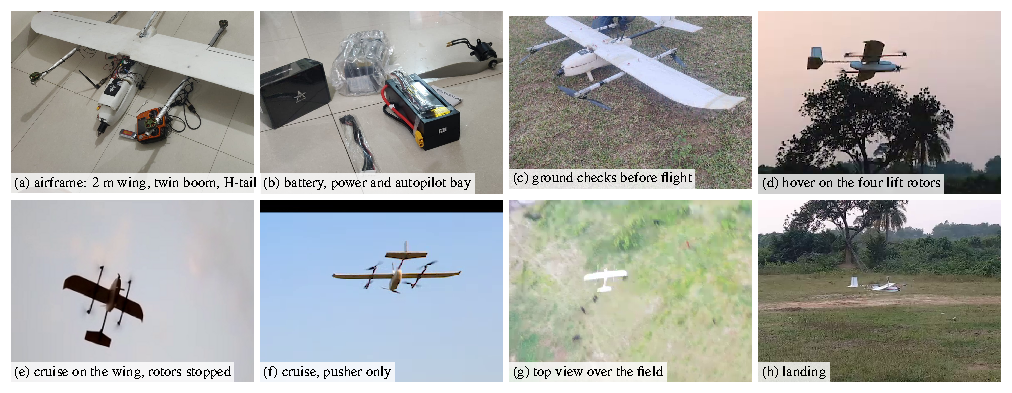
\includegraphics[width=\textwidth]{fig04_hardware.pdf}
\caption{The quadplane: airframe, power and autopilot bay, ground checks, hover on the lift rotors, cruise on the wing with the rotors stopped, cruise on the pusher, top view over the field, and landing.}\label{fig:aircraft}
\end{figure*}

\subsection{Identified model and parameter box}
The parameters of \eqref{eq:model} were identified from the PX4 log of a flight with several hand-offs, released as a dataset~\cite{Dony2026data}: the polar $(C_{L0},C_{L\alpha},C_{D0},k)$ from the lift and drag balances of the cruise segments anchored to the computational-fluid-dynamics polar of the wing, the attitude-loop rate and gain $(\kappa,\gth)$ from the pitch response to the setpoint, the thrust maps $(k_{\mathrm c},k_{\mathrm r})$ from the throttle-to-acceleration balances and the actuator lags from the transitions. Table~\ref{tab:box} lists the nominal values and the intervals that define the box $\Theta$: two standard deviations of the identification for the polar, the range of attitude-loop settings of the autopilot for $\kappa$ and $\gth$, and $\pm50\%$ of the lags and the identified spread of the thrust maps for the actuators. The power of the rotors follows the momentum-theory law $P_{\mathrm r}=c_{\mathrm r}T_{\mathrm r}^{3/2}$ through the measured hover power and the pusher power the linear law $P_{\mathrm c}=c_{\mathrm c}T_{\mathrm c}$ through the measured cruise power.
\begin{table}[t]\centering\footnotesize
\caption{Nominal parameters and the box $\Theta$ identified from the flight log.}\label{tab:box}
\setlength{\tabcolsep}{2.5pt}\scriptsize
\begin{tabular}{lcc|lcc}\toprule
parameter & nominal & interval & parameter & nominal & interval\\\midrule
$C_{L0}$ & 1.141 & $\pm0.144$ & $\kappa$ [1/s] & 2.0 & $[0.67,5.0]$\\
$C_{L\alpha}$ [1/rad] & 3.12 & $\pm25\%$ & $\gth$ & 1.0 & $[0.9,1.0]$\\
$C_{D0}$ & 0.133 & $\pm0.044$ & $\lambda_{\mathrm c}$ [1/s] & 2.0 & $[1.33,4.0]$\\
$k$ & 0.060 & $\pm25\%$ & $\lambda_{\mathrm r}$ [1/s] & 6.67 & $[4.44,13.3]$\\
$\overline T_{\mathrm c}$ [N] & 30.3 & $\beta_{\mathrm c}\in[0.78,1.22]$ & $\overline T_{\mathrm r}$ [N] & 118.7 & $\beta_{\mathrm r}\in[0.85,1.15]$\\
\bottomrule\end{tabular}\end{table}
The constraints are $\bar\alpha=\SI{5}{\degree}$ (inside the range verified unstalled in cruise), $\theta\in[-15,20]^\circ$, $\gamma\in[-15,15]^\circ$, $V_{\min}=\SI{4}{m/s}$, $K_L=\numKL{}$, $\dot\gamma_{\lim}=\SI{\numGdLim}{rad/s}$, the input box $|\thsp|\le\SI{30}{\degree}$, $T^{\mathrm c}_{\mathrm c}\in[0,\SI{30.3}{N}]$, $T^{\mathrm c}_{\mathrm r}\in[0,\SI{118.7}{N}]$ and the step bounds $\bar\delta=(\SI{4}{\degree},\SI{0.75}{N},\SI{4}{N})$ per \SI{50}{ms}. The corridor runs from the hover-exit airspeed $\rho_0=\SI{6}{m/s}$ to the cruise airspeed $\rho_{\mathrm c}=\SI{15}{m/s}$.

\subsection{Simulator, training and the safety module}\label{sec:num}
The differentiable model integrates \eqref{eq:model} with a Runge--Kutta step of two substeps per sample in PyTorch~\cite{Paszke2019} and the linear polar; the evaluation plant uses five substeps in NumPy and folds the lift curve beyond the stall angles of $10^\circ$ and $-14^\circ$ with a post-stall slope of \SI{-2}{/rad} and a drag rise, so that a policy that leaves the linear range is punished by the plant rather than rewarded by the model. HOT has $L=\numL{}$ tokens of width $d=\numD{}$, $N=\numBlocks{}$ blocks of \numHeads{} heads, \numParams{} parameters, and is trained for \numIters{} iterations of batch \numBatch{} with Adam, learning rate \numLr{} with cosine decay, gradient norm clipped at $1$, weights $(w_E,w_B,w_A,w_S)=(\numWE,\numWB,\numWA,\numWS)$ in \eqref{eq:loss}, gust standard deviation \SI{1}{m/s} and the noise of Table~\ref{tab:noise} on the window; the curriculum grows the horizon from \SI{3}{s} to \SI{15}{s} over the first $60\%$ of the iterations. The lift-safety module uses the plant set of the \numPlantsOnline{} vertices of the fast parameters and the lift-curve offset with \numSamplesOnline{} interior samples online, the backup gains $k_\gamma=\numKgam$, $k_{\mathrm r}=\numKr$~N per rad/s per step, the reference band $[\numRlo,\numRhi]$~rad/s, the lead $\tau_{\mathrm b}=\numTauB$~s, the pusher loop $k_{\mathrm c}=\numKc$~N per m/s$^2$ per step, $k_V=\numKv$~/s, $\bar a=\numAmax$~m/s$^2$ on the corridor $[\numVblo,\numVbhi]$~m/s, the horizon $H=\numH{}$ samples, the margins $m=(\numMargins)$, the settled neighbourhood $\mathcal C$: lift fraction in $[\numClfLo,\numClfHi]$, $|\gamma|\le\numCgam^\circ$, $|\dot\gamma|\le\numCgd$~rad/s, $\alpha\in[\numCalLo,\numCalHi]^\circ$, $V\in[\numCvLo,\numCvHi]$~m/s and $|\dot V|\le\numCvd$~m/s$^2$, and the measurement bound $\varepsilon=(\numEps)$. Assumption~\ref{ass:settle} was verified over the full plant set of \numPlantsFull{} plants; the one-step gain of Lemma~\ref{lem:corner} is \numKrGain{}.
\begin{table}[t]\centering\footnotesize
\caption{Sensor-noise standard deviations applied to the window during training and in the noise cell.}\label{tab:noise}
\begin{tabular}{lccccc}\toprule
& $V$ [m/s] & $\gamma$ [deg] & $\theta$ [deg] & $T_{\mathrm c}$ [N] & $T_{\mathrm r}$ [N]\\\midrule
level 1 & 0.3 & 0.5 & 0.3 & 0.6 & 2.4\\
\bottomrule\end{tabular}\end{table}

\subsection{PX4 firmware in the loop}
The autopilot firmware (PX4 v1.17) runs in software-in-the-loop with its simulation-in-hardware plant configured to the identified aircraft: mass, inertia, rotor thrust and lag, the wing with the polar of Table~\ref{tab:box}, the tail and the pusher lag. The firmware's estimator, attitude and rate loops, control allocation and offboard interface are unchanged; HOT runs as an offboard node that receives the states over MAVLink at \SI{100}{Hz}, sends the pitch setpoint and the rotor collective as an attitude target and the pusher command as an actuator-set command, and re-plans every \SI{50}{ms}. The network evaluates in \hotEvalMs{}~ms and the safety check takes \hotCheckMs{}~ms on average (\hotCheckMaxMs{}~ms at most) in interpreted code on one core, so the loop runs at real time on average and the simulation is slowed to half speed to keep every update inside its period.



% ---- sec8_experiments ----
\section{Experiments}\label{sec:experiments}
\subsection{Set-up, baselines, metrics and statistics}
Every controller runs in the same loop: the plant \eqref{eq:model} with the true parameters, the state delivered with the noise of Table~\ref{tab:noise} scaled by the noise level of the cell, the commands sampled every \SI{50}{ms} and rate-limited, \SI{20}{s} of simulation. Table~\ref{tab:controllers} lists the nine controllers. The threshold rule (THR) reproduces the autopilot logic; the fixed lift-sharing schedule (SCH) follows the nominal trim of the current airspeed with a pusher loop on the airspeed and a rotor loop on the flight-path rate; the gain-scheduled PID (GS-PID) schedules its gains on the airspeed; the model predictive controller (MPC) solves a nominal-model tracking problem on a \SI{4}{s} horizon by sequential conic programming; the feed-forward (MLP) and recurrent (LSTM) policies use the bounded head of HOT and are trained by the same physics-informed procedure; HOT$-$LSM is the transformer without the safety module; PPO~\cite{Schulman2017} and SAC~\cite{Haarnoja2018} are trained with Stable-Baselines3~\cite{Raffin2021} on the same plant family with the negative of \eqref{eq:loss} as the reward. Metrics: the time to the target airspeed (first entry within \SI{0.3}{m/s}), the energy of the identified power model, the minimum lift fraction, the maximum angle of attack, the extreme flight-path angles and the minimum sink rate, the percentage of samples with a violated constraint, the intervention rate of the safety module and the wall time per update. Statistics: mean and standard deviation over plants and seeds, the Wilcoxon signed-rank test at $p<0.05$ against HOT ($+/=/-$ counts of the cells in which HOT is better, equal or worse) and the Friedman mean rank~\cite{Demsar2006}.
\begin{table}[t]\centering\footnotesize
\caption{Controllers compared.}\label{tab:controllers}
\setlength{\tabcolsep}{4pt}
\begin{tabular}{llcc}\toprule
label & controller & learned & guarantee\\\midrule
THR & autopilot threshold rule & -- & --\\
SCH & fixed lift-sharing schedule & -- & --\\
GS-PID & gain-scheduled PID & -- & --\\
MPC & nominal-model MPC, \SI{4}{s} horizon & -- & nominal plant\\
MLP & feed-forward policy, bounded head & \checkmark & --\\
LSTM & recurrent policy on the window & \checkmark & --\\
HOT$-$LSM & transformer without the safety module & \checkmark & --\\
PPO, SAC & reinforcement learning, same reward & \checkmark & --\\
HOT & this article & \checkmark & Theorem~\ref{thm:main}\\
\bottomrule\end{tabular}\end{table}

\subsection{Training}\label{sec:trainres}
%% Fig: training curves (loss terms, violation rate, reached fraction) for HOT, MLP, LSTM; text with numbers

% ---- res_training ----
Fig.~\ref{fig:train} shows the training of HOT, the feed-forward and the recurrent policy under the same procedure: the time term, the barrier term, the fraction of episodes that reach the target within the horizon and the plant-head loss over the iterations. The barrier term falls by \trainBarrierDrop{} over the training and the reached fraction rises to \trainReached{} at the final horizon of \SI{15}{s}; the plant-head loss falls to \trainAux{}, i.e.\ the context token has learned to carry the plant. Training took \trainWallMin{}~min on four processor cores.
\begin{figure*}[t]\centering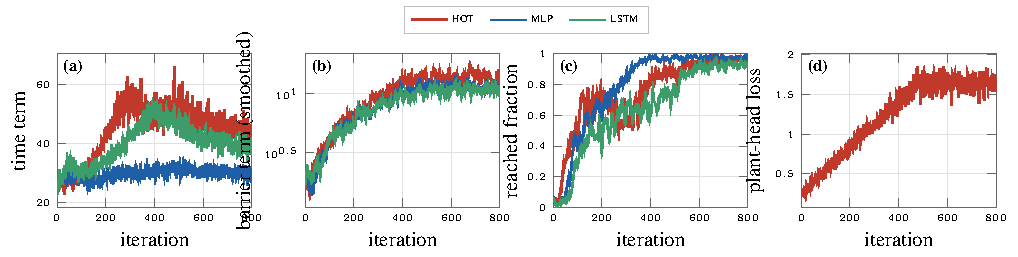
\includegraphics[width=\textwidth]{fig05_training.pdf}
\caption{Training curves under the physics-informed procedure: (a) time term; (b) barrier term; (c) fraction of episodes that reach the target within the curriculum horizon; (d) plant-head loss of HOT.}\label{fig:train}
\end{figure*}


\subsection{Nominal transitions}\label{sec:nominal}
%% Fig: nominal front and back transitions, all controllers (V, lift fraction, alpha, commands); Table: metrics

% ---- res_nominal ----
Fig.~\ref{fig:nominal} shows both transitions on the identified plant for every controller and Table~\ref{tab:nominal} the metrics. HOT reaches cruise in \hotFrontT{}~s and the hover-exit airspeed in \hotBackT{}~s with the lift fraction never below \hotFrontLf{} and \hotBackLf{}, the angle of attack below \hotFrontAl{}$^\circ$ and \hotBackAl{}$^\circ$, and \hotFrontEnergy{}~Wh and \hotBackEnergy{}~Wh of energy; the safety module intervened at \hotFrontInterv{} of the \hotFrontUpd{} front updates and \hotBackInterv{} of the \hotBackUpd{} back updates, and the same policy without the module, HOT$-$LSM, flies the same times (\hotnfFrontT{} and \hotnfBackT{}~s) but crosses the pitch box on the way. The threshold rule is fast in the front transition because it cuts the rotors as soon as the airspeed crosses its threshold, at the price of the lowest lift fraction of all controllers, \thrFrontLf{}; the schedule and the gain-scheduled PID keep the lift near unity but need \schFrontT{}~s and \pidFrontT{}~s in the front and 11 to 15~s in the back transition; the nominal-model MPC keeps the lift fraction at unity and takes \mpcFrontT{}~s with its \SI{4}{s} horizon and rate limits. The feed-forward and recurrent policies, run with the same module, take \mlpFrontT{}~s and \lstmFrontT{}~s in the front transition and hold less lift; SAC reaches the target in \sacFrontT{}~s and \sacBackT{}~s, and PPO does not reach cruise within the window on the identified plant, its rotor command oscillating between its bounds (Fig.~\ref{fig:nominal}d).
\begin{figure}[t]\centering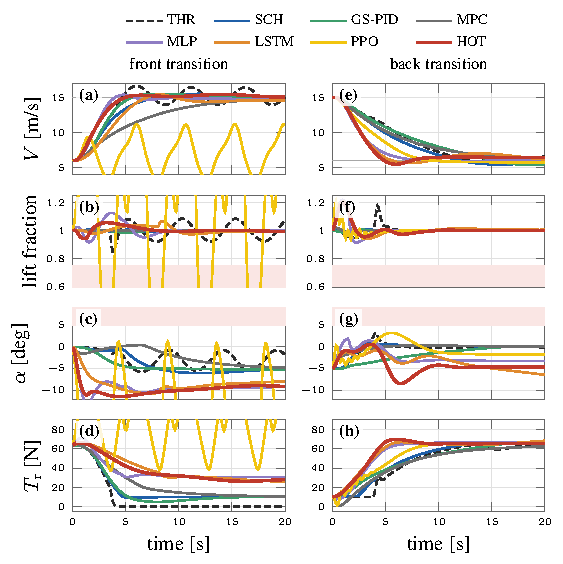
\includegraphics[width=\columnwidth]{fig06_nominal.pdf}
\caption{Nominal front (left) and back (right) transitions: airspeed, lift fraction with the \SI{75}{\percent} bound, angle of attack with its bound, rotor thrust, for eight controllers (SAC, close to PPO, is in Table~\ref{tab:nominal}).}\label{fig:nominal}
\end{figure}
\begin{table*}[t]\centering\footnotesize
\caption{Metrics on the identified plant.}\label{tab:nominal}

% ---- tables/nominal ----
\begin{tabular}{l|cccc|cccc}\toprule
& \multicolumn{4}{c|}{front transition ($6\to15$ m/s)} & \multicolumn{4}{c}{back transition ($15\to6$ m/s)}\\
controller & time [s] & energy [Wh] & min $\lf$ & max $\alpha$ [deg] & time [s] & energy [Wh] & min $\lf$ & max $\alpha$ [deg]\\\midrule
THR & 4.6 & 2.99 & 0.84 & -0.0 & 12.2 & 3.51 & 0.95 & 3.2\\
SCH & 7.2 & 3.38 & 0.99 & -0.0 & 11.3 & 3.77 & 0.98 & 0.8\\
GS-PID & 5.2 & 3.32 & 0.99 & -0.0 & 14.5 & 3.56 & 0.98 & -0.0\\
MPC & 18.4 & 3.39 & 1.00 & 0.4 & 19.5 & 3.60 & 1.00 & 0.3\\
MLP & 3.8 & 4.02 & 0.92 & -0.1 & 6.9 & 4.51 & 0.92 & 1.9\\
LSTM & 6.6 & 4.16 & 0.97 & -0.0 & 5.2 & 4.87 & 0.94 & -0.8\\
HOT$-$LSM & 4.0 & 4.17 & 0.94 & -0.2 & 4.7 & 4.51 & 0.96 & 0.6\\
PPO & -- & 8.94 & 0.32 & 1.2 & 8.2 & 4.03 & 0.94 & 3.2\\
SAC & 7.3 & 3.01 & 0.91 & -0.3 & 4.9 & 4.30 & 0.94 & 4.7\\
\textbf{HOT} & 4.5 & 4.21 & 0.94 & -0.2 & 4.7 & 4.51 & 0.96 & 0.6\\
\bottomrule\end{tabular}

\end{table*}


\subsection{Generalisation across the plant family}\label{sec:cross}
%% Fig: box plots per metric over the unseen plants, Friedman ranks; Table: Wilcoxon +/=/-

% ---- res_cross ----
Table~\ref{tab:cross} and Fig.~\ref{fig:cross} report the \numCross{} unseen plants of the box, none of which was seen in training and none of which is known to any controller, with a front and a back transition each. HOT reaches the target band within the \SI{20}{s} window on \hotCrossFrontReached{} of the \hotCrossFrontN{} front and \hotCrossBackReached{} of the \hotCrossBackN{} back transitions, in a median of \hotCrossFrontTmed{}~s and \hotCrossBackTmed{}~s when it does, keeps the lift fraction above \hotCrossLf{} on every plant and violates no constraint on any of them; the module intervened at \hotCrossFrontIntervPct{}\% of the front and \hotCrossBackIntervPct{}\% of the back updates. The Wilcoxon test on the time to target is significant at $p<0.05$ in favour of HOT against every controller except its own unfiltered version, and the Friedman mean rank over the \numFriedmanN{} transitions flown by all controllers is \hotCrossRank{} for HOT against \bestOtherCrossRank{} for the best alternative, \bestOtherCrossName{}. The price of the guarantee is energy, about one watt-hour more than the classical controllers, spent by the rotors during the shorter transition, and the lift fraction, which the schedule and the gain-scheduled PID hold at 0.97 by taking twice the time. The transitions that finish after the \SI{20}{s} window are the ones on which the module holds the rotors longer than the policy asks, on strong-wing plants whose light-wing counterparts are still in the retained set, or on which the policy settles just above the band after a backup step; they are safe and slower, not failures of the guarantee. The transformer without the module, HOT$-$LSM, reaches \hotnfCrossReached{} of the transitions in \hotnfCrossT{}~s but violates a constraint on \hotnfCrossViol{}\% of the samples over the family, the threshold rule on \thrCrossViol{}\%, the schedule on \schCrossViol{}\% and PPO on \ppoCrossViol{}\%; the gain-scheduled PID and the MPC violate nothing but take \pidCrossT{} and \mpcCrossT{}~s, and the MPC reaches \mpcCrossReached{} of its transitions. The module is therefore what turns the fastest policy into a safe one.
\begin{table*}[t]\centering\footnotesize
\caption{Generalisation across the plant family: \numCross{} unseen plants, front and back transitions, mean $\pm$ standard deviation; W: Wilcoxon signed-rank test against HOT ($+$: HOT better, $=$: no difference, $-$: HOT worse, $p<0.05$); rank: Friedman mean rank on the time to target (lower is better).}\label{tab:cross}

% ---- tables/cross ----
\begin{tabular}{l|c|cc|cc|cc|c|c}\toprule
controller & reached & time [s] & W & energy [Wh] & W & min $\lf$ & W & viol.\ [\%] & rank\\\midrule
THR & 0.96 & 8.0$\pm$3.9 & $+$ & 3.18$\pm$0.67 & $-$ & 0.88$\pm$0.06 & $+$ & 1.6 & 3.82\\
SCH & 0.87 & 9.4$\pm$2.9 & $+$ & 3.62$\pm$0.44 & $-$ & 0.97$\pm$0.03 & $-$ & 2.5 & 5.24\\
GS-PID & 0.95 & 9.7$\pm$4.5 & $+$ & 3.50$\pm$0.34 & $-$ & 0.97$\pm$0.03 & $-$ & 0.0 & 5.06\\
MPC & 0.50 & 15.1$\pm$3.4 & $+$ & 3.44$\pm$0.22 & $-$ & 0.96$\pm$0.04 & $-$ & 0.0 & 7.28\\
HOT$-$LSM & 0.98 & 5.2$\pm$2.1 & $-$ & 4.39$\pm$0.28 & $=$ & 0.92$\pm$0.07 & $=$ & 1.6 & 1.89\\
PPO & 0.50 & 8.3$\pm$1.1 & $+$ & 6.48$\pm$2.49 & $+$ & 0.60$\pm$0.31 & $+$ & 36.6 & 5.61\\
SAC & 0.87 & 5.9$\pm$2.0 & $+$ & 3.66$\pm$0.67 & $-$ & 0.91$\pm$0.03 & $+$ & 0.3 & 3.86\\
\textbf{HOT} & 0.89 & 5.5$\pm$2.5 &  & 4.38$\pm$0.25 &  & 0.94$\pm$0.02 &  & 0.0 & 3.24\\
\bottomrule\end{tabular}

\end{table*}
\begin{figure*}[t]\centering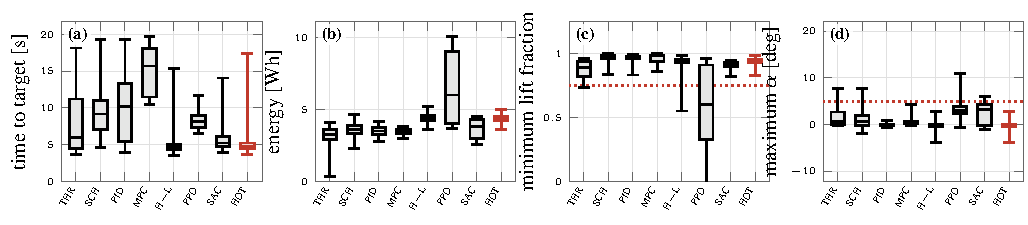
\includegraphics[width=\textwidth]{fig07_cross.pdf}
\caption{Distribution over the \numCross{} unseen plants of the time to target, the energy, the minimum lift fraction and the maximum angle of attack for each controller (boxes: quartiles; whiskers: extremes; dotted: bounds).}\label{fig:cross}
\end{figure*}


\subsection{Outside the box, gusts and noise}\label{sec:robust}

% ---- res_robust ----
Table~\ref{tab:robust} and Fig.~\ref{fig:sweeps} extend the test beyond the training distribution: \numOutbox{} plants drawn from a box enlarged by \SI{50}{\percent} about its centre, vertical gusts of 0.25 to \SI{1.5}{m/s} standard deviation and sensor noise of half to twice the identified level, ten seeds each. Outside the box HOT reaches the band on \hotOutFrontReached{} of \hotOutFrontN{} front and \hotOutBackReached{} of \hotOutBackN{} back transitions with the lift fraction above \hotOutLf{} and no violation; the module intervenes at \hotOutFrontIntervPct{}\% of the front updates, and \hotOutFrontStalledNoInt{} front and \hotOutBackStalledNoInt{} back misses happen without any intervention, which is the policy itself leaving its training distribution. The threshold rule reaches \thrOutReached{} of these transitions with the lift fraction at \thrOutLf{} and \thrOutViol{}\% of the samples in violation. Gusts lie outside the plant family that the certificate covers: the backup is rolled out without the gust, and a gust moves the flight path by more than the measurement bound $\varepsilon$ in one step, so at 1 and \SI{1.5}{m/s} the module applies the backup itself on \hotGustStrongUnverShare{}\% of its interventions (\hotGustStrongInterv{}\% of the updates). At \SI{0.25}{m/s} nothing is violated; at 1 and \SI{1.5}{m/s} the angle-of-attack and lift bounds are crossed on \hotGustStrongViol{}\% of the samples, against \pidGustOneViol{} and \pidGustOneHalfViol{}\% for the gain-scheduled PID, \thrGustOneHalfViol{}\% for the threshold rule and \sacGustOneHalfViol{}\% for SAC at \SI{1.5}{m/s}, while HOT keeps the highest minimum lift fraction of all controllers under the strongest gust, \hotGustOneHalfLf{} against \thrGustOneHalfLf{} and \sacGustOneHalfLf{}. Enlarging $\varepsilon$ by the gust bound restores the coverage of Lemma~\ref{lem:cons} at the price of a larger retained set. Under sensor noise the module keeps every constraint at every level; the back transition is unaffected (\hotNoiseTwoBackReached{} of 10 within the window at twice the noise, median \hotNoiseTwoBackTmed{}~s), whereas the front transition slows with the noise, median \hotNoiseOneFrontTmed{}~s at the identified level and \hotNoiseTwoFrontTmed{}~s with \hotNoiseTwoFrontReached{} of 10 within the window at twice the level: the noisy window slows the acceleration while the module intervenes at only \hotNoiseInterv{}\% of the updates.
\begin{table*}[t]\centering\footnotesize
\caption{Outside the box, gusts and noise: fraction of transitions that reach the target within \SI{20}{s}, minimum lift fraction (mean $\pm$ standard deviation) and fraction of samples in violation of a constraint.}\label{tab:robust}

% ---- tables/robust ----
\begin{tabular}{l|ccc|ccc|ccc}\toprule
& \multicolumn{3}{c|}{outside the box} & \multicolumn{3}{c|}{gusts} & \multicolumn{3}{c}{noise}\\
controller & reached & min $\lf$ & viol.\ [\%] & reached & min $\lf$ & viol.\ [\%] & reached & min $\lf$ & viol.\ [\%]\\\midrule
THR & 0.89 & 0.87$\pm$0.07 & 1.3 & 0.96 & 0.78$\pm$0.17 & 9.3 & 1.00 & 0.89$\pm$0.06 & 0.0\\
SCH & 0.78 & 0.95$\pm$0.05 & 4.3 & 0.96 & 0.83$\pm$0.15 & 9.8 & 1.00 & 0.97$\pm$0.01 & 0.0\\
GS-PID & 0.78 & 0.95$\pm$0.05 & 0.0 & 0.84 & 0.84$\pm$0.14 & 3.6 & 1.00 & 0.97$\pm$0.01 & 0.0\\
PPO & 0.48 & -3.31$\pm$19.95 & 38.4 & 0.50 & 0.54$\pm$0.30 & 37.4 & 0.50 & 0.62$\pm$0.30 & 35.9\\
SAC & 0.84 & 0.90$\pm$0.04 & 0.3 & 1.00 & 0.79$\pm$0.16 & 6.0 & 1.00 & 0.91$\pm$0.02 & 0.1\\
\textbf{HOT} & 0.66 & 0.92$\pm$0.05 & 0.0 & 0.89 & 0.87$\pm$0.08 & 8.4 & 0.87 & 0.95$\pm$0.01 & 0.0\\
\bottomrule\end{tabular}

\end{table*}
\begin{figure*}[t]\centering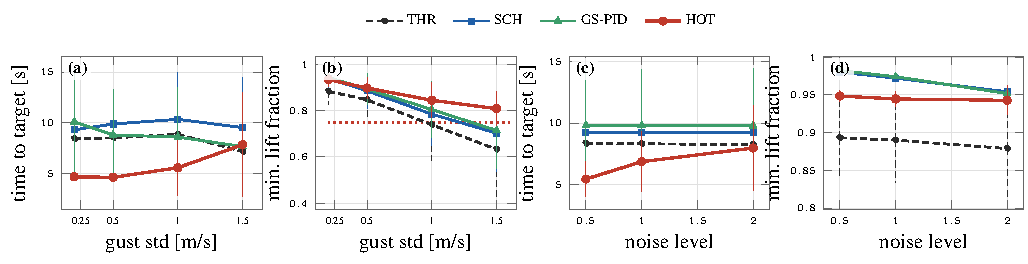
\includegraphics[width=\textwidth]{fig09_sweeps.pdf}
\caption{Time to target and minimum lift fraction against the gust standard deviation (a, b) and the sensor-noise level (c, d), mean and standard deviation over ten seeds and both transitions.}\label{fig:sweeps}
\end{figure*}


\subsection{From the states recorded in flight}\label{sec:replay}

% ---- res_replay ----
The dataset~\cite{Dony2026data} records the aircraft's own hand-offs under the threshold rule, including a front transition in which the rotors were cut early and the wing lost lift for three seconds, and a back transition that ran to a high angle of attack. Fig.~\ref{fig:replay} starts HOT from the state recorded \SI{2.7}{s} before that rotor cut, at \SI{5.4}{m/s} and climbing, and from the state recorded as the back transition began, at \SI{13.4}{m/s} with the rotors off. Both states lie outside the training distribution of trims. From the front state HOT keeps the lift fraction above \hotReplayFrontLf{} where the recorded flight lost its lift, the module holding the rotors through \hotReplayFrontInterv{} certified interventions in the low-speed climb so that the wing is never asked for lift it cannot give, and the aircraft accelerates to cruise beyond the \SI{20}{s} window; from the back state it spins the rotors up within the step bound, keeps the angle of attack below \hotReplayBackAl{}$^\circ$, where the recorded flight went to $36^\circ$, and reaches the band in \hotReplayBackT{}~s with \hotReplayBackInterv{} interventions.
\begin{figure}[t]\centering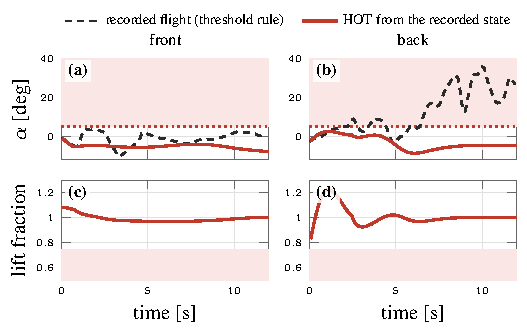
\includegraphics[width=\columnwidth]{fig10_replay.pdf}
\caption{Angle of attack and lift fraction of HOT started from the states recorded in flight (solid) beside the recorded continuation under the threshold rule (dashed), front (left) and back (right).}\label{fig:replay}
\end{figure}


\subsection{PX4 firmware in the loop}\label{sec:sil}

% ---- res_sil ----
Fig.~\ref{fig:sil} shows both transitions with the PX4 firmware in the loop, from the trims reached under the same commands. The front transition reaches cruise in \silFrontT{}~s and the back transition enters the hover-exit band at \silBackT{}~s, both slower than on the identified model (Section~\ref{sec:nominal}): the firmware's aircraft carries the drag of its fuselage and tail plates and a slower attitude loop than the identified one, and the policy, which is not told which plant it is flying, commands the pitch and the pusher it learned for the box, so the airspeed follows the drag of the aircraft it meets; in the back transition the last metre per second is bled by drag alone, with the pusher at zero and the rotors near hover thrust, which takes ten seconds. The angle of attack stays within $[\silFrontAlMin^\circ,\silFrontAlMax^\circ]$ and $[\silBackAlMin^\circ,\silBackAlMax^\circ]$, the flight path within $\silFrontGam^\circ$ and $\silBackGam^\circ$, and the lift fraction evaluated on the identified model never falls below \silFrontLf{} and \silBackLf{}. The pitch setpoint carries the noise of the firmware's airspeed estimate, which the attitude loop filters out of the pitch; the module certified every command (\silFrontInterv{} interventions in \silFrontUpd{} and \silBackInterv{} in \silBackUpd{} updates). The update, network and check together, took \silUpdMs{}~ms on average in the loop, on a processor shared with the parallel evaluations.
\begin{figure*}[t]\centering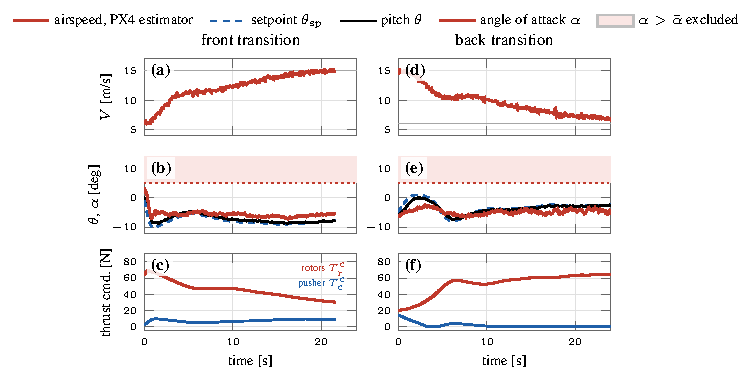
\includegraphics[width=0.72\textwidth]{fig11_sil.pdf}
\caption{Closed loop with the PX4 firmware in software-in-the-loop, front (left) and back (right) transitions: airspeed from the autopilot's estimator, pitch setpoint sent to the attitude loop with the pitch and angle of attack it produced, rotor and pusher commands.}\label{fig:sil}
\end{figure*}


\subsection{Ablations and parameter analysis}\label{sec:ablation}

% ---- res_ablation ----
Fig.~\ref{fig:ablation} evaluates the architecture on the first \numAblPlants{} plants of the cross-plant cell, both transitions, with the bare policy and with the module: HOT with one module removed, the feed-forward and recurrent policies trained by the same procedure, and reduced sizes. The reduced variants and the module ablations were trained for 500 iterations, HOT, MLP and LSTM for 800. Without the physics features the bare policy reaches the band on \ablNoPhysReached{}\% of the transitions against \ablFullReached{}\% for HOT and violates on \ablNoPhysViol{}\% of the samples; without the auxiliary head the context token still resolves the parameters (mean $R^2$ \ablNoAuxRtwo{} against \interpRtwoMean{}), which the pooled physics features carry on their own, and the policy reaches \ablNoAuxReached{}\%. The feed-forward policy trained by the same physics-informed procedure, with the same physics features and previous command, also flies the box (\ablMlpReached{}\% of the transitions in a median of \ablMlpTmed{}~s), and the recurrent policy \ablLstmReached{}\% in \ablLstmTmed{}~s: the training procedure and the physics features of Section~\ref{sec:method} transfer to every architecture, and the history-conditioned transformer adds to them the plant estimate of Section~\ref{sec:interp}, which the feed-forward policy cannot form. With the module every variant is free of violations. A window of 8 samples, a width of 32 and a single block reach \ablLsmallReached{}, \ablDsmallReached{} and \ablBoneReached{}\% of the transitions bare at the shorter training budget.
\begin{figure*}[t]\centering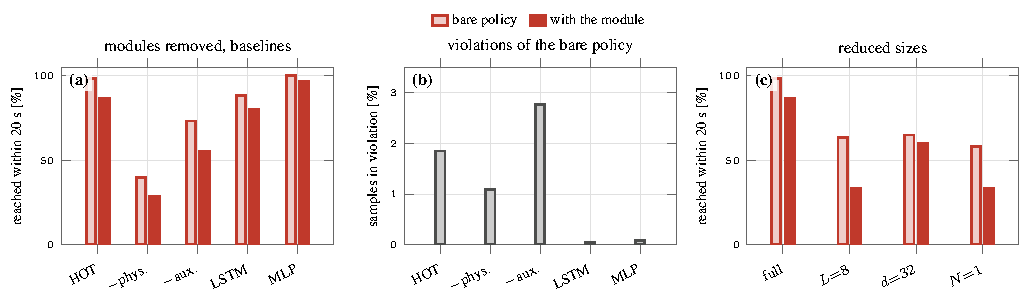
\includegraphics[width=0.8\textwidth]{fig12_ablation.pdf}
\caption{Ablations and parameter analysis on \numAblPlants{} unseen plants, both transitions: (a) fraction of transitions that reach the band within \SI{20}{s}, bare policy and with the module, for HOT, HOT without the physics features, without the auxiliary head, the LSTM and the MLP; (b) fraction of samples in violation for the bare policies; (c) reach fraction of the reduced sizes (window 8, width 32, one block; trained for 500 iterations).}\label{fig:ablation}
\end{figure*}


\subsection{Interpretability: attention and the context token}\label{sec:interp}

% ---- res_interp ----
Fig.~\ref{fig:interp} looks inside the plant-inference attention. The attention of the context token over the window is nearly uniform, between \interpAttMin{} and \interpAttMax{} against $1/L=\interpAttUniform{}$ (a): the token pools the whole window rather than a few samples, and the plant information sits in the pooled physics features. Panels (b) and (c) follow the $R^2$ between the context-token estimate and the true parameter along the transition on the unseen plants: each parameter is resolved while the response that reveals it is inside the window and released once the window has slid past it. The lift-curve offset is read off the wing-borne trim at the start of the back transition ($R^2=\interpRtwoCLzero{}$ at \interpTCLzero{}~s), the rotor gain once the rotors respond in the \interpTrBetaR{} transition ($\interpRtwoBetaR{}$ at \interpTBetaR{}~s), the attitude-loop rate from the first pitch response in the \interpTrKappa{} transition ($\interpRtwoKappa{}$ at \interpTKappa{}~s) and the lift-curve slope during the acceleration ($\interpRtwoCLa{}$ at \interpTCLa{}~s); the drag parameters, which act on the airspeed slowly, are not resolved ($R^2$ at most \interpRtwoCDzero{}). The estimates are shrunk towards the centre of the box by the measurement noise, to \interpShrinkCLzero{} of the true spread for $C_{L0}$, as a least-squares head under noise should be, so (d) and (e) show them standardised. A sliding window implies this forgetting; the ablation of the auxiliary head (Section~\ref{sec:ablation}) measures what the estimate is worth to the policy.
\begin{figure*}[t]\centering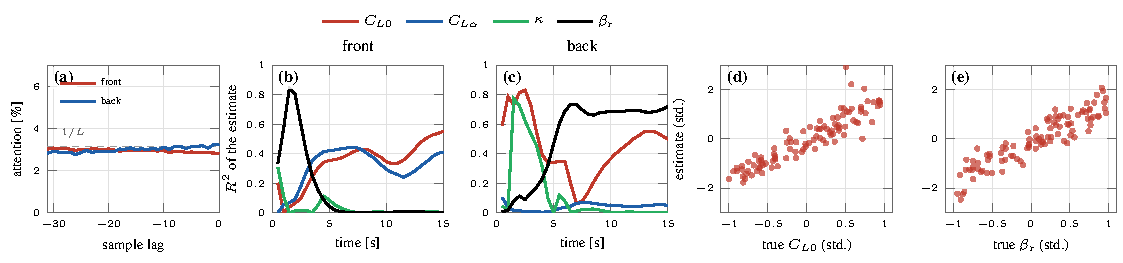
\includegraphics[width=\textwidth]{fig13_interp.pdf}
\caption{Interpretability on the unseen plants: (a) attention of the context token over the window, front and back, against the uniform weight $1/L$; (b), (c) $R^2$ of the context-token estimate of the lift-curve offset, the lift-curve slope, the attitude-loop rate and the rotor gain against the true values along the front and the back transition; (d), (e) standardised estimates against the standardised true values at the time of the best $R^2$.}\label{fig:interp}
\end{figure*}


\subsection{Time cost}\label{sec:time}

% ---- res_time ----
Table~\ref{tab:time} lists the update times on one core of the development computer in interpreted Python. The network evaluates in \hotEvalMs{}~ms; the safety check takes \hotCheckMs{}~ms on average and \hotCheckMaxMs{}~ms at most with the online plant set, most of it in the rollouts of the backup, and it is skipped when the network command has already been certified at the previous step for a state that has not moved; the nominal-model MPC needs \mpcStepMs{}~ms per update.
\begin{table}[t]\centering\footnotesize
\caption{Properties of transition controllers and learned controllers with safety (\checkmark: yes, --: no).}\label{tab:compare}
\setlength{\tabcolsep}{2.5pt}
\begin{tabular}{lcccccc}\toprule
& \rotatebox{90}{learned policy} & \rotatebox{90}{plant family} & \rotatebox{90}{implicit identification} & \rotatebox{90}{lift guarantee} & \rotatebox{90}{lagged actuators} & \rotatebox{90}{flight-identified}\\\midrule
Threshold rule~\cite{PX4docs} & -- & -- & -- & -- & -- & \checkmark\\
Gain-scheduled / hierarchical~\cite{Lyu2017,Verling2016} & -- & -- & -- & -- & -- & \checkmark\\
Optimised manoeuvre~\cite{Maqsood2012} & -- & -- & -- & -- & -- & --\\
Transition MPC~\cite{Li2018,Allenspach2020,Bauersfeld2021} & -- & -- & -- & -- & -- & \checkmark\\
Adaptive VTOL control~\cite{Dong2020} & -- & \checkmark & -- & -- & -- & --\\
Approximate MPC~\cite{Hertneck2018,Karg2020,Chen2018} & \checkmark & -- & -- & -- & -- & --\\
Predictive / backup safety filters~\cite{Wabersich2021,Gurriet2020} & \checkmark & -- & -- & -- & -- & --\\
Domain randomisation, adaptation~\cite{Peng2018,Kumar2021} & \checkmark & \checkmark & \checkmark & -- & -- & --\\
This article & \checkmark & \checkmark & \checkmark & \checkmark & \checkmark & \checkmark\\
\bottomrule\end{tabular}\end{table}
\begin{table}[t]\centering\footnotesize
\caption{Update time per controller (one core, interpreted code).}\label{tab:time}
\begin{tabular}{lc}\toprule
controller & time per update\\\midrule
threshold rule & \thrUs{}~\si{\micro\second}\\
schedule, GS-PID & \schUs{}~\si{\micro\second}, \pidUs{}~\si{\micro\second}\\
MPC (sequential conic programming) & \mpcStepMs{}~ms\\
HOT network & \hotEvalMs{}~ms\\
HOT safety check (mean, max) & \hotCheckMs{}, \hotCheckMaxMs{}~ms\\
\bottomrule\end{tabular}\end{table}


\subsection{Comparison with previous work}\label{sec:compare}

% ---- res_compare ----
Table~\ref{tab:compare} places HOT against the transition controllers and the learned controllers of Section~\ref{sec:related} on the properties that this article set out to combine. The autopilot rule and the gain-scheduled and optimised transitions of the VTOL literature plan nothing online and carry no guarantee on the lift; model predictive transition controllers plan online but on one nominal model; approximate model predictive control and the safety-filter literature certify a learned or a nominal command on one plant; domain-randomised policies generalise across plants but without a constraint guarantee. HOT is the only entry that learns a single policy over a plant family, infers the plant it is flying from its own history, guarantees the lift margin, the angle of attack, the flight path and the sink rate for every plant of the verified set with lagged actuators and the attitude loop inside the plant, and is validated on a flight-identified aircraft with the autopilot firmware in the loop.





% ---- sec9_conclusion ----
\section{Conclusion}\label{sec:conclusion}
This article asked whether one neural policy can fly the hand-off of a quadplane for every aircraft of an identified parameter box, without being told which one it is flying, and with a guarantee on the lift it carries. The answer is HOT, a history-conditioned transformer whose context token infers the plant from the last $L$ autopilot samples, trained by backpropagation through the differentiable model identified from the flight log under domain randomisation, gusts and noise, and wrapped by a lift-safety module that certifies each command against a backup manoeuvre over the plant set and the plants consistent with the observed motion. The module is recursively feasible and keeps the lift fraction, the angle of attack, the flight path and the sink rate within bounds for every plant of the verified set; a verifiable decrease condition gives practical convergence; the context token resolves the plant parameters while the responses that reveal them are inside the window. On the identified aircraft HOT completes the front transition in \hotFrontT{}~s and the back transition in \hotBackT{}~s with the lift fraction never below \hotFrontLf{}; on \numCross{} unseen plants it reaches the target on \hotCrossReached{} of the transitions without a constraint violation, where the feed-forward, recurrent and reinforcement-learning policies violate on up to \maxOtherCrossViol{}\% of the samples; it keeps its guarantee outside the box, under gusts and noise and from the states recorded in flight, and it flies both transitions with the PX4 firmware in the loop.

Future work follows three lines. Training the policy through the module, so that certified commands become part of its experience, will remove the few transitions that finish after the window. The guarantee is stated over a finite plant set and extends to the box through a Lipschitz argument whose constant is estimated rather than bounded; a verified bound, or a set-membership contraction of the box itself rather than of a sample, will close this gap, and enlarging the measurement bound by the gust bound extends the certificate to gusts. The backup manoeuvre and the settled neighbourhood were verified numerically over twenty-second rollouts; an analytic invariance proof for the level-off law is within reach for the frozen-wing model. Lateral motion, wind and the landing flare are outside the longitudinal model; the same architecture and module apply once the plant family is extended to them, and the compiled controller on the aircraft's companion computer is the next flight test.



% ---- backmatter ----
\section*{CRediT authorship contribution statement}
\textbf{Md Nur-A-Adam Dony:} Conceptualization, Methodology, Software, Formal analysis, Investigation, Data curation, Validation, Visualization, Writing -- original draft, Writing -- review \& editing, Project administration. \textbf{Md Azizul Islam:} Resources, Investigation, Validation, Writing -- review \& editing.
\section*{Declaration of competing interest}
The authors declare that they have no known competing financial interests or personal relationships that could have appeared to influence the work reported in this paper.
\section*{Funding}
This research did not receive any specific grant from funding agencies in the public, commercial, or not-for-profit sectors.
\section*{Declaration of generative AI and AI-assisted technologies in the manuscript preparation process}
During the preparation of this work the authors used Claude (Anthropic) in order to assist with the drafting of text, the preparation of figures and the implementation of the simulation and analysis code. After using this tool, the authors reviewed and edited the content as needed and take full responsibility for the content of the published article.
\section*{Data availability}
The flight-test telemetry and the CFD data of the aircraft are available in the dataset repository cited in the article~\cite{Dony2026data}. The identified model, the controller, the training and evaluation code, the trained networks, the PX4 software-in-the-loop set-up and the results of every experiment are available at \url{https://github.com/AdamDony/quadplane-hot} (archived with a DOI upon acceptance).


\bibliographystyle{elsarticle-num}

% ---- refs ----
\begin{thebibliography}{00}
\bibitem{Meier2015} L.~Meier, D.~Honegger, and M.~Pollefeys, PX4: A node-based multithreaded open source robotics framework for deeply embedded platforms, in Proc. IEEE Int. Conf. Robot. Autom., 2015, pp. 6235--6240.
\bibitem{PX4docs} PX4 Development Team, PX4 user guide: VTOL transitions, \url{https://docs.px4.io/}, accessed Sep. 2026.
\bibitem{Lyu2017} X.~Lyu, H.~Gu, J.~Zhou, Z.~Li, S.~Shen, and F.~Zhang, A hierarchical control approach for a quadrotor tail-sitter VTOL UAV and experimental verification, in Proc. IEEE/RSJ Int. Conf. Intell. Robots Syst., 2017, pp. 5135--5141.
\bibitem{Verling2016} S.~Verling, B.~Weibel, M.~Boosfeld, K.~Alexis, M.~Burri, and R.~Siegwart, Full attitude control of a VTOL tailsitter UAV, in Proc. IEEE Int. Conf. Robot. Autom., 2016, pp. 3006--3012.
\bibitem{Maqsood2012} A.~Maqsood and T.~H. Go, Optimization of transition maneuvers through aerodynamic vectoring, Aerosp. Sci. Technol., vol. 23, no. 1, pp. 363--371, 2012.
\bibitem{Li2018} B.~Li, W.~Zhou, J.~Sun, C.-Y. Wen, and C.-K. Chen, Development of model predictive controller for a tail-sitter VTOL UAV in hover flight, Sensors, vol. 18, no. 9, p. 2859, 2018.
\bibitem{Allenspach2020} M.~Allenspach, K.~Bodie, M.~Brunner, L.~Rinsoz, Z.~Taylor, M.~Kamel, R.~Siegwart, and J.~Nieto, Design and optimal control of a tiltrotor micro-aerial vehicle for efficient omnidirectional flight, Int. J. Robot. Res., vol. 39, no. 10--11, pp. 1305--1325, 2020.
\bibitem{Bauersfeld2021} L.~Bauersfeld, L.~Spannagl, G.~J.~J. Ducard, and C.~H. Onder, MPC flight control for a tilt-rotor VTOL aircraft, IEEE Trans. Aerosp. Electron. Syst., vol. 57, no. 4, pp. 2395--2409, 2021.
\bibitem{Dong2020} W.~Dong, M.~N.-A.-A. Dony, and M.~Rafat, Tracking control of vertical taking-off and landing vehicles with parametric uncertainty, Int. J. Adapt. Control Signal Process., vol. 34, pp. 1294--1307, 2020.
\bibitem{Dony2020acc} M.~N.-A.-A. Dony, M.~Rafat, and W.~Dong, Distributed command filtered robust tracking control of wave-adaptive modular vessel with uncertainty, in Proc. Amer. Control Conf., Denver, CO, USA, 2020, pp. 2118--2123.
\bibitem{Dony2021jae} M.~N.-A.-A. Dony and W.~Dong, Distributed robust formation flying and attitude synchronization of spacecraft, J. Aerosp. Eng., vol. 34, no. 3, 2021.
\bibitem{Dony2021thesis} M.~N.-A.-A. Dony, Robust distributed formation control of UAVs with higher-order dynamics, M.S. thesis, The University of Texas Rio Grande Valley, Edinburg, TX, USA, 2021, ScholarWorks @ UTRGV, \url{https://scholarworks.utrgv.edu/etd/856}.
\bibitem{Dony2025rs} M.~N.-A.-A. Dony and B.~Arhin, Safe model-free Q-learning for discrete-time fully cooperative multi-input systems with state and control constraints via control barrier functions, Research Square, preprint, 2025.
\bibitem{Dony2025ieom} M.~N.-A.-A. Dony, M.~E. Khallil, and M.~S. Ali, Adaptive reinforcement learning with control barrier functions for safe state avoidance in discrete event systems, in Proc. 8th IEOM Bangladesh Int. Conf. Ind. Eng. Oper. Manag., Dhaka, Bangladesh, Dec. 2025, doi: 10.46254/BA08.20250300.
\bibitem{Dony2026data} M.~N.-A.-A. Dony, M.~A. Islam, M.~Hasan, and S.~G.~M. Hossain, Quadplane PX4 flight data: flight-test telemetry and CFD data for a small quadplane VTOL, dataset, \url{https://github.com/AdamDony/quadplane-px4-flight-data}, 2026.
\bibitem{Anderson2017} J.~D. Anderson, Fundamentals of Aerodynamics, 6th ed. New York, NY, USA: McGraw-Hill, 2017.
\bibitem{Selig1997} M.~S. Selig and J.~J. Guglielmo, High-lift low Reynolds number airfoil design, J. Aircr., vol. 34, no. 1, pp. 72--79, 1997.
\bibitem{Kaufmann2023} E.~Kaufmann, L.~Bauersfeld, A.~Loquercio, M.~M\"uller, V.~Koltun, D.~Scaramuzza, Champion-level drone racing using deep reinforcement learning, Nature 620 (2023) 982--987.
\bibitem{Song2023} Y.~Song, A.~Romero, M.~M\"uller, V.~Koltun, D.~Scaramuzza, Reaching the limit in autonomous racing: optimal control versus reinforcement learning, Sci. Robot. 8 (2023) eadg1462.
\bibitem{Hertneck2018} M.~Hertneck, J.~K\"ohler, S.~Trimpe, F.~Allg\"ower, Learning an approximate model predictive controller with guarantees, IEEE Control Syst. Lett. 2 (2018) 543--548.
\bibitem{Karg2020} B.~Karg, S.~Lucia, Efficient representation and approximation of model predictive control laws via deep learning, IEEE Trans. Cybern. 50 (2020) 3866--3878.
\bibitem{Chen2018} S.~Chen, K.~Saulnier, N.~Atanasov, D.~D. Lee, V.~Kumar, G.~J. Pappas, M.~Morari, Approximating explicit model predictive control using constrained neural networks, in: Proc. Amer. Control Conf., 2018, pp. 1520--1527.
\bibitem{Ames2019} A.~D. Ames, S.~Coogan, M.~Egerstedt, G.~Notomista, K.~Sreenath, P.~Tabuada, Control barrier functions: theory and applications, in: Proc. Eur. Control Conf., 2019, pp. 3420--3431.
\bibitem{Wabersich2021} K.~P. Wabersich, M.~N. Zeilinger, A predictive safety filter for learning-based control of constrained nonlinear dynamical systems, Automatica 129 (2021) 109597.
\bibitem{Gurriet2020} T.~Gurriet, M.~Mote, A.~Singletary, P.~Nilsson, E.~Feron, A.~D. Ames, A scalable safety critical control framework for nonlinear systems, IEEE Access 8 (2020) 187249--187275.
\bibitem{Alshiekh2018} M.~Alshiekh, R.~Bloem, R.~Ehlers, B.~K\"onighofer, S.~Niekum, U.~Topcu, Safe reinforcement learning via shielding, in: Proc. AAAI Conf. Artif. Intell., 2018, pp. 2669--2678.
\bibitem{Hewing2020} L.~Hewing, K.~P. Wabersich, M.~Menner, M.~N. Zeilinger, Learning-based model predictive control: toward safe learning in control, Annu. Rev. Control Robot. Auton. Syst. 3 (2020) 269--296.
\bibitem{Brunke2022} L.~Brunke, M.~Greeff, A.~W. Hall, Z.~Yuan, S.~Zhou, J.~Panerati, A.~P. Schoellig, Safe learning in robotics: from learning-based control to safe reinforcement learning, Annu. Rev. Control Robot. Auton. Syst. 5 (2022) 411--444.
\bibitem{Tobin2017} J.~Tobin, R.~Fong, A.~Ray, J.~Schneider, W.~Zaremba, P.~Abbeel, Domain randomization for transferring deep neural networks from simulation to the real world, in: Proc. IEEE/RSJ Int. Conf. Intell. Robots Syst., 2017, pp. 23--30.
\bibitem{Peng2018} X.~B. Peng, M.~Andrychowicz, W.~Zaremba, P.~Abbeel, Sim-to-real transfer of robotic control with dynamics randomization, in: Proc. IEEE Int. Conf. Robot. Autom., 2018, pp. 3803--3810.
\bibitem{Kumar2021} A.~Kumar, Z.~Fu, D.~Pathak, J.~Malik, RMA: rapid motor adaptation for legged robots, in: Proc. Robotics: Science and Systems, 2021.
\bibitem{Chen2021DT} L.~Chen, K.~Lu, A.~Rajeswaran, K.~Lee, A.~Grover, M.~Laskin, P.~Abbeel, A.~Srinivas, I.~Mordatch, Decision transformer: reinforcement learning via sequence modeling, in: Adv. Neural Inf. Process. Syst., Vol. 34, 2021, pp. 15084--15097.
\bibitem{Janner2021} M.~Janner, Q.~Li, S.~Levine, Offline reinforcement learning as one big sequence modeling problem, in: Adv. Neural Inf. Process. Syst., Vol. 34, 2021, pp. 1273--1286.
\bibitem{Lee2023} J.~N. Lee, A.~Xie, A.~Pacchiano, Y.~Chandak, C.~Finn, O.~Nachum, E.~Brunskill, Supervised pretraining can learn in-context reinforcement learning, in: Adv. Neural Inf. Process. Syst., Vol. 36, 2023.
\bibitem{Vaswani2017} A.~Vaswani, N.~Shazeer, N.~Parmar, J.~Uszkoreit, L.~Jones, A.~N. Gomez, {\L}.~Kaiser, I.~Polosukhin, Attention is all you need, in: Adv. Neural Inf. Process. Syst., Vol. 30, 2017, pp. 5998--6008.
\bibitem{Yun2020} C.~Yun, S.~Bhojanapalli, A.~S. Rawat, S.~J. Reddi, S.~Kumar, Are transformers universal approximators of sequence-to-sequence functions?, in: Proc. Int. Conf. Learn. Represent., 2020.
\bibitem{Schulman2017} J.~Schulman, F.~Wolski, P.~Dhariwal, A.~Radford, O.~Klimov, Proximal policy optimization algorithms, arXiv:1707.06347 (2017).
\bibitem{Haarnoja2018} T.~Haarnoja, A.~Zhou, P.~Abbeel, S.~Levine, Soft actor-critic: off-policy maximum entropy deep reinforcement learning with a stochastic actor, in: Proc. Int. Conf. Mach. Learn., 2018, pp. 1861--1870.
\bibitem{Raffin2021} A.~Raffin, A.~Hill, A.~Gleave, A.~Kanervisto, M.~Ernestus, N.~Dormann, Stable-Baselines3: reliable reinforcement learning implementations, J. Mach. Learn. Res. 22 (2021) 1--8.
\bibitem{Demsar2006} J.~Dem\v{s}ar, Statistical comparisons of classifiers over multiple data sets, J. Mach. Learn. Res. 7 (2006) 1--30.
\bibitem{Diehl2005} M.~Diehl, H.~G. Bock, J.~P. Schl\"oder, A real-time iteration scheme for nonlinear optimization in optimal feedback control, SIAM J. Control Optim. 43 (2005) 1714--1736.
\bibitem{Goulart2024} P.~J. Goulart, Y.~Chen, Clarabel: an interior-point solver for conic programs with quadratic objectives, arXiv:2405.12762 (2024).
\bibitem{Bobiti2018} R.~Bobiti, M.~Lazar, Automated-sampling-based stability verification and DOA estimation for nonlinear systems, IEEE Trans. Autom. Control 63 (2018) 3659--3674.
\bibitem{Paszke2019} A.~Paszke, S.~Gross, F.~Massa, A.~Lerer, J.~Bradbury, G.~Chanan, T.~Killeen, Z.~Lin, N.~Gimelshein, L.~Antiga, A.~Desmaison, A.~K\"opf, E.~Yang, Z.~DeVito, M.~Raison, A.~Tejani, S.~Chilamkurthy, B.~Steiner, L.~Fang, J.~Bai, S.~Chintala, PyTorch: an imperative style, high-performance deep learning library, in: Adv. Neural Inf. Process. Syst., Vol. 32, 2019, pp. 8024--8035.
\end{thebibliography}


\end{document}
